\newpage\null\par
\section{实验四\hspace{1em}声环境质量现状评价}
\subsection{教学目的与要求}
\noindent\textbf{教学目的:}通过噪声源参数现状数据实例来进行声环境质量评价。

\noindent\textbf{教学要求:}
\begin{enumerate}
    \item 掌握声环境质量现状调查监测计划的设置方法,制定某校区的声环境质量现状监测方案并进行评价;
    \item 掌握声环境预测软件EIAN2.0和Surfer绘图软件在声环境质量评价中的应用,熟悉等声值线图绘制的基本方法。利用EIAN和Sufer软件自行拟定参数(声源分贝、预测网格步长等)绘制出一个声源(点源或者面源)的分布衰减等声线图(图形优化后),并附上主要操作步骤截图。
    \item 鼓励使用Cadna/A 软件进行影响预测。
\end{enumerate}


\subsection{实验报告背景}
\subsubsection{监测点布设}
监测点布设本项目噪声监测共布设4个点(如图 \ref{fig:Acoustic environment monitoring dot map}、\ref{fig:Sound_environment_monitoring_points} 和表 \ref{tab:Acoustic environment monitoring location information} 所示)。按国家规定的噪声测试规范要求进行昼间和夜间环境噪声监测。

\begin{table}[H]
    \centering
    \caption{声环境监测布点位置信息}
    \begin{tabular}{cccc}
        \toprule
        图像点位 & 位置名称 & 经度 & 纬度 \\
        \midrule
        点1 & 体育馆二楼篮球场 & $104^{\circ}41'26.58''$ & $28^{\circ}48'58.51''$ \\
        点2 & 图书馆二楼中心 & $104^{\circ}41'32.01''$ & $28^{\circ}49'3.43''$ \\
        点3 & 教学楼甲一楼 & $104^{\circ}41'32.88''$ & $28^{\circ}49'7.96''$ \\
        点4 & 一期食堂一楼 & $104^{\circ}41'40.11''$ & $28^{\circ}48'59.28''$ \\
        \bottomrule
    \end{tabular}
    \label{tab:Acoustic environment monitoring location information}
\end{table}

\begin{figure}[H]
    \centering
    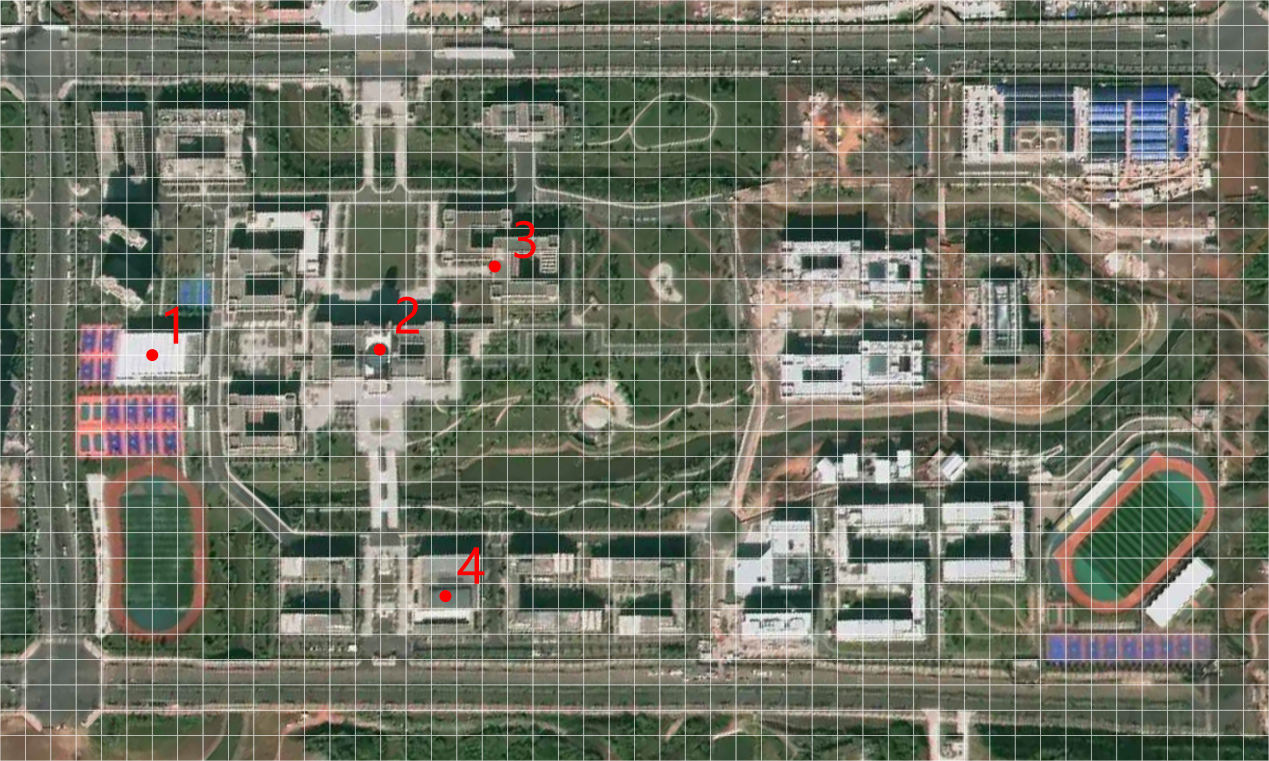
\includegraphics[width=\textwidth]{figures/Acoustic environment monitoring dot map.png}
    \caption{声环境监测布点图}
    \label{fig:Acoustic environment monitoring dot map}
\end{figure}

\begin{figure}[H]
    \centering
    \begin{subfigure}[htb]{0.48\textwidth}
        \centering
        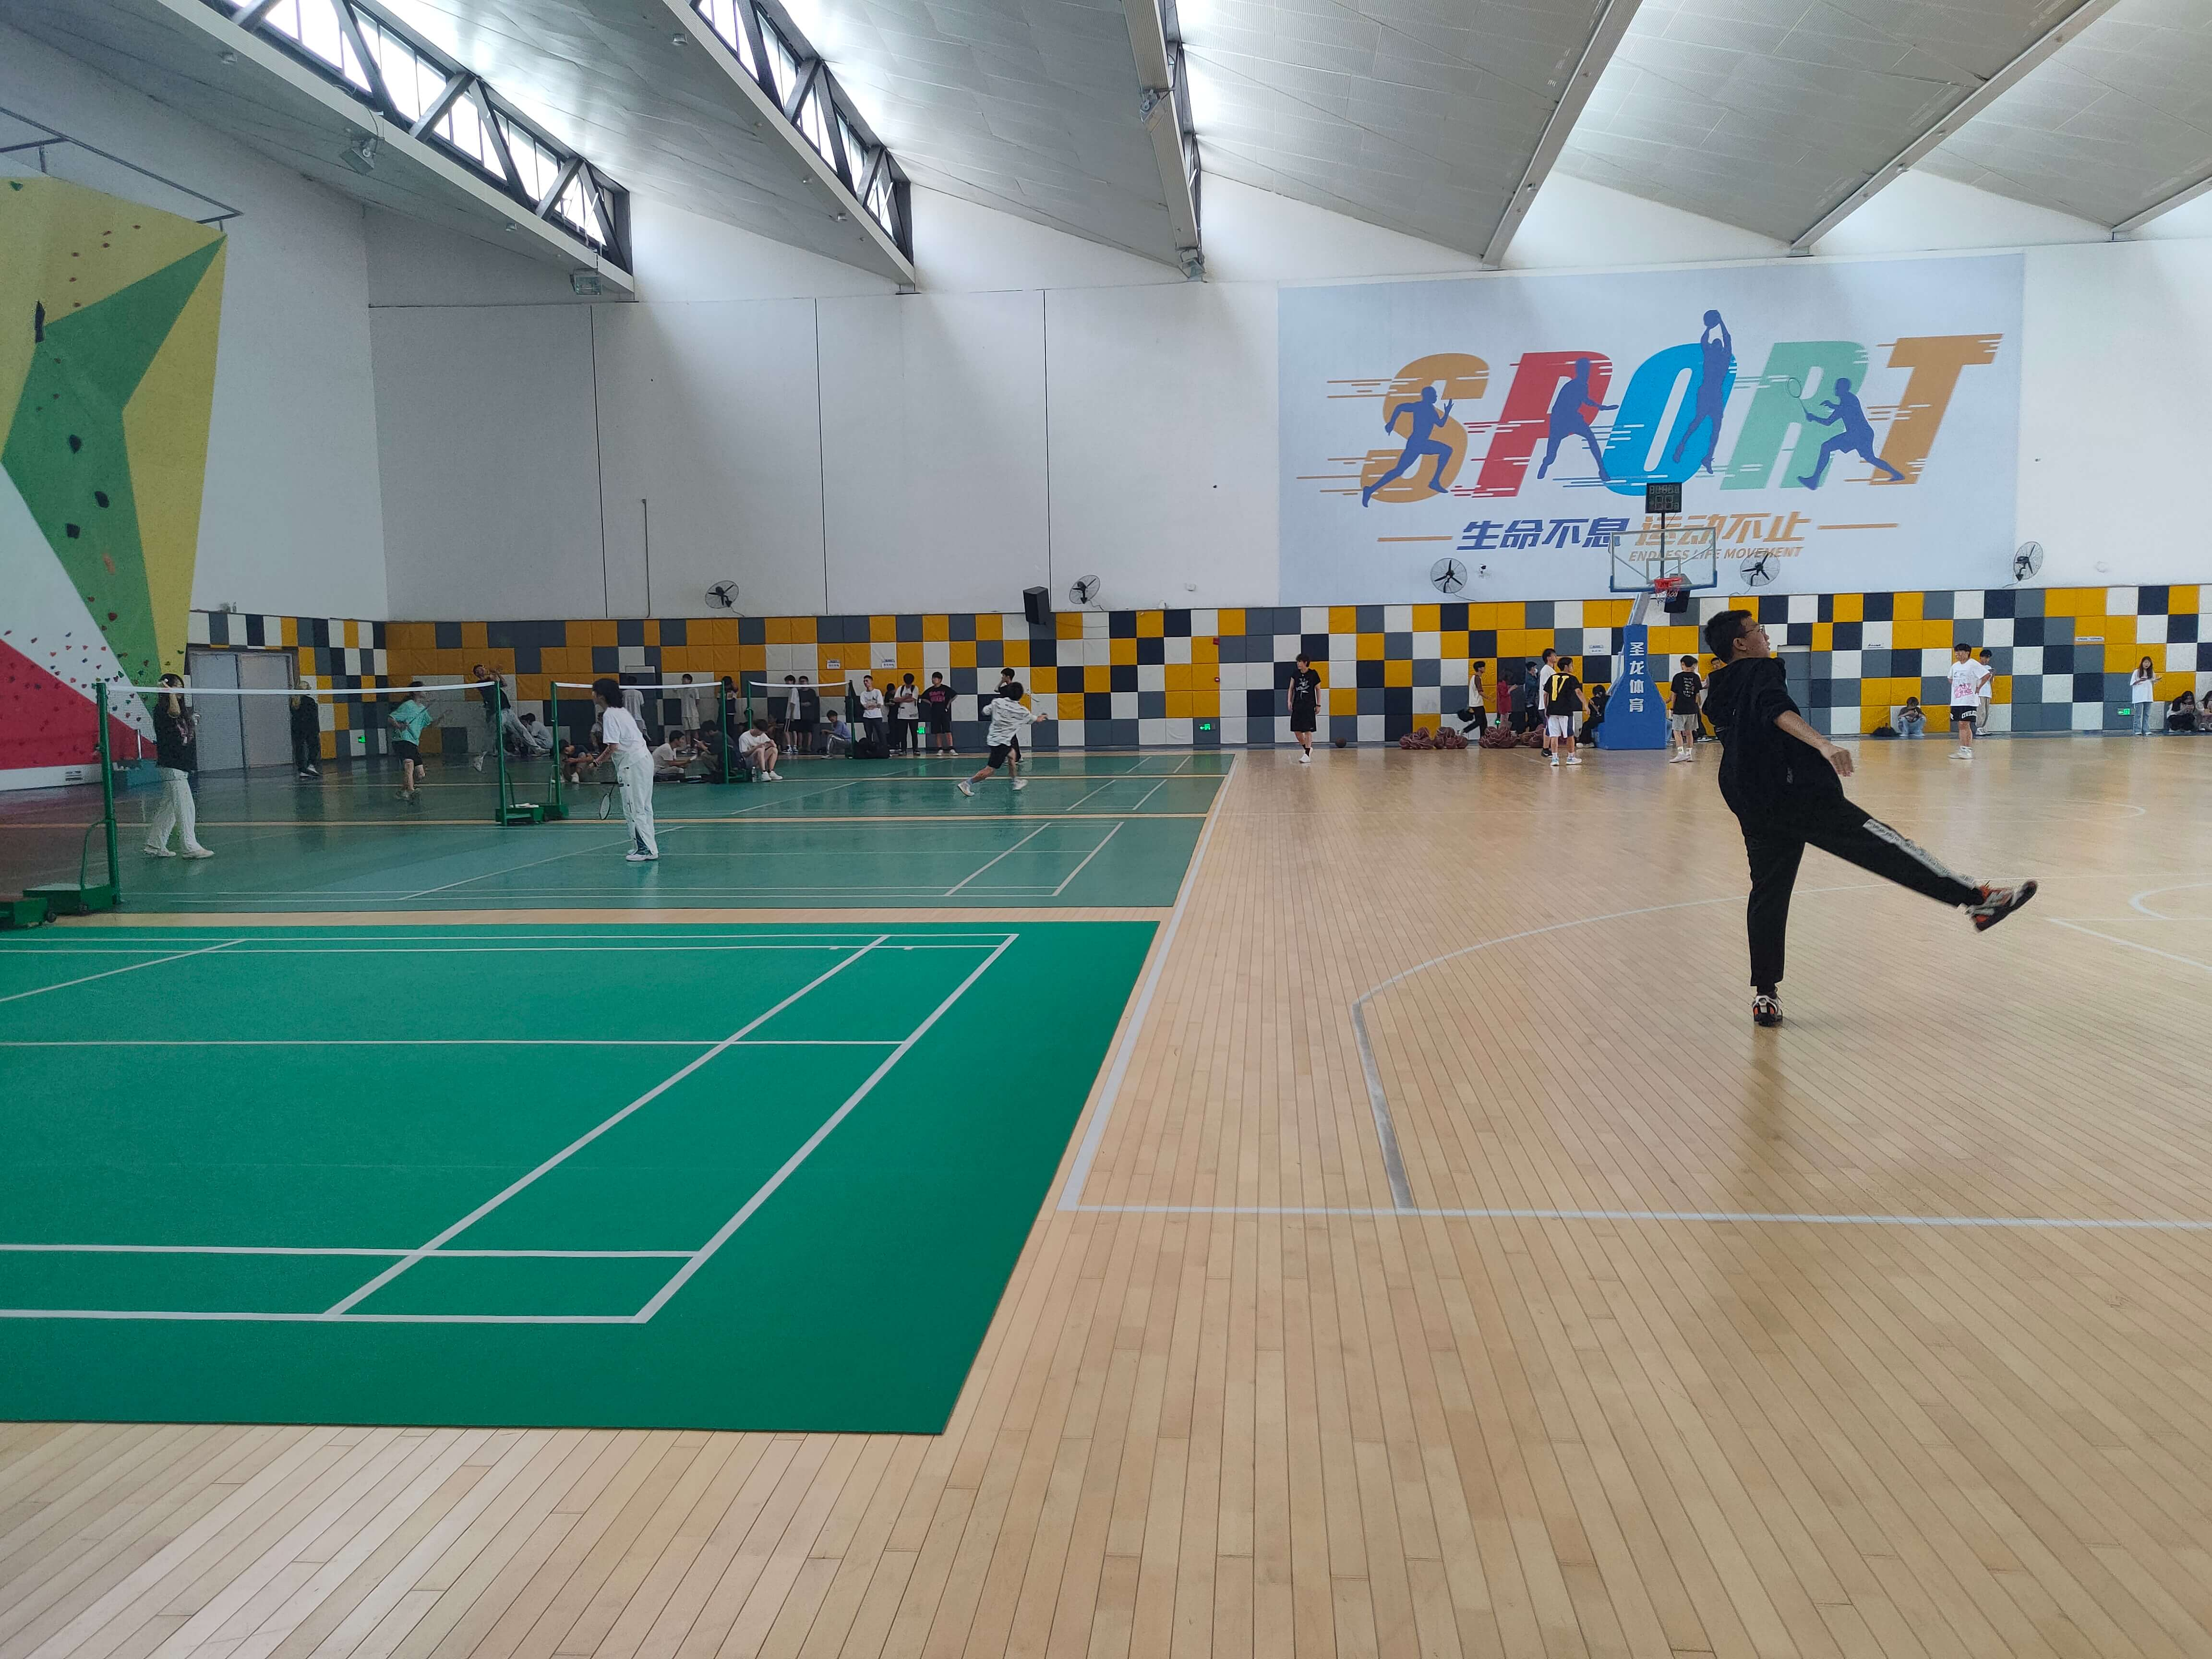
\includegraphics[width=\textwidth]{figures/Monitoring_point_-_basketball_court_on_the_second_floor_of_the_gymnasium.jpg}
        \caption{体育馆二楼篮球场}
    \end{subfigure}
    \hfill
    \begin{subfigure}[htb]{0.48\textwidth}
        \centering
        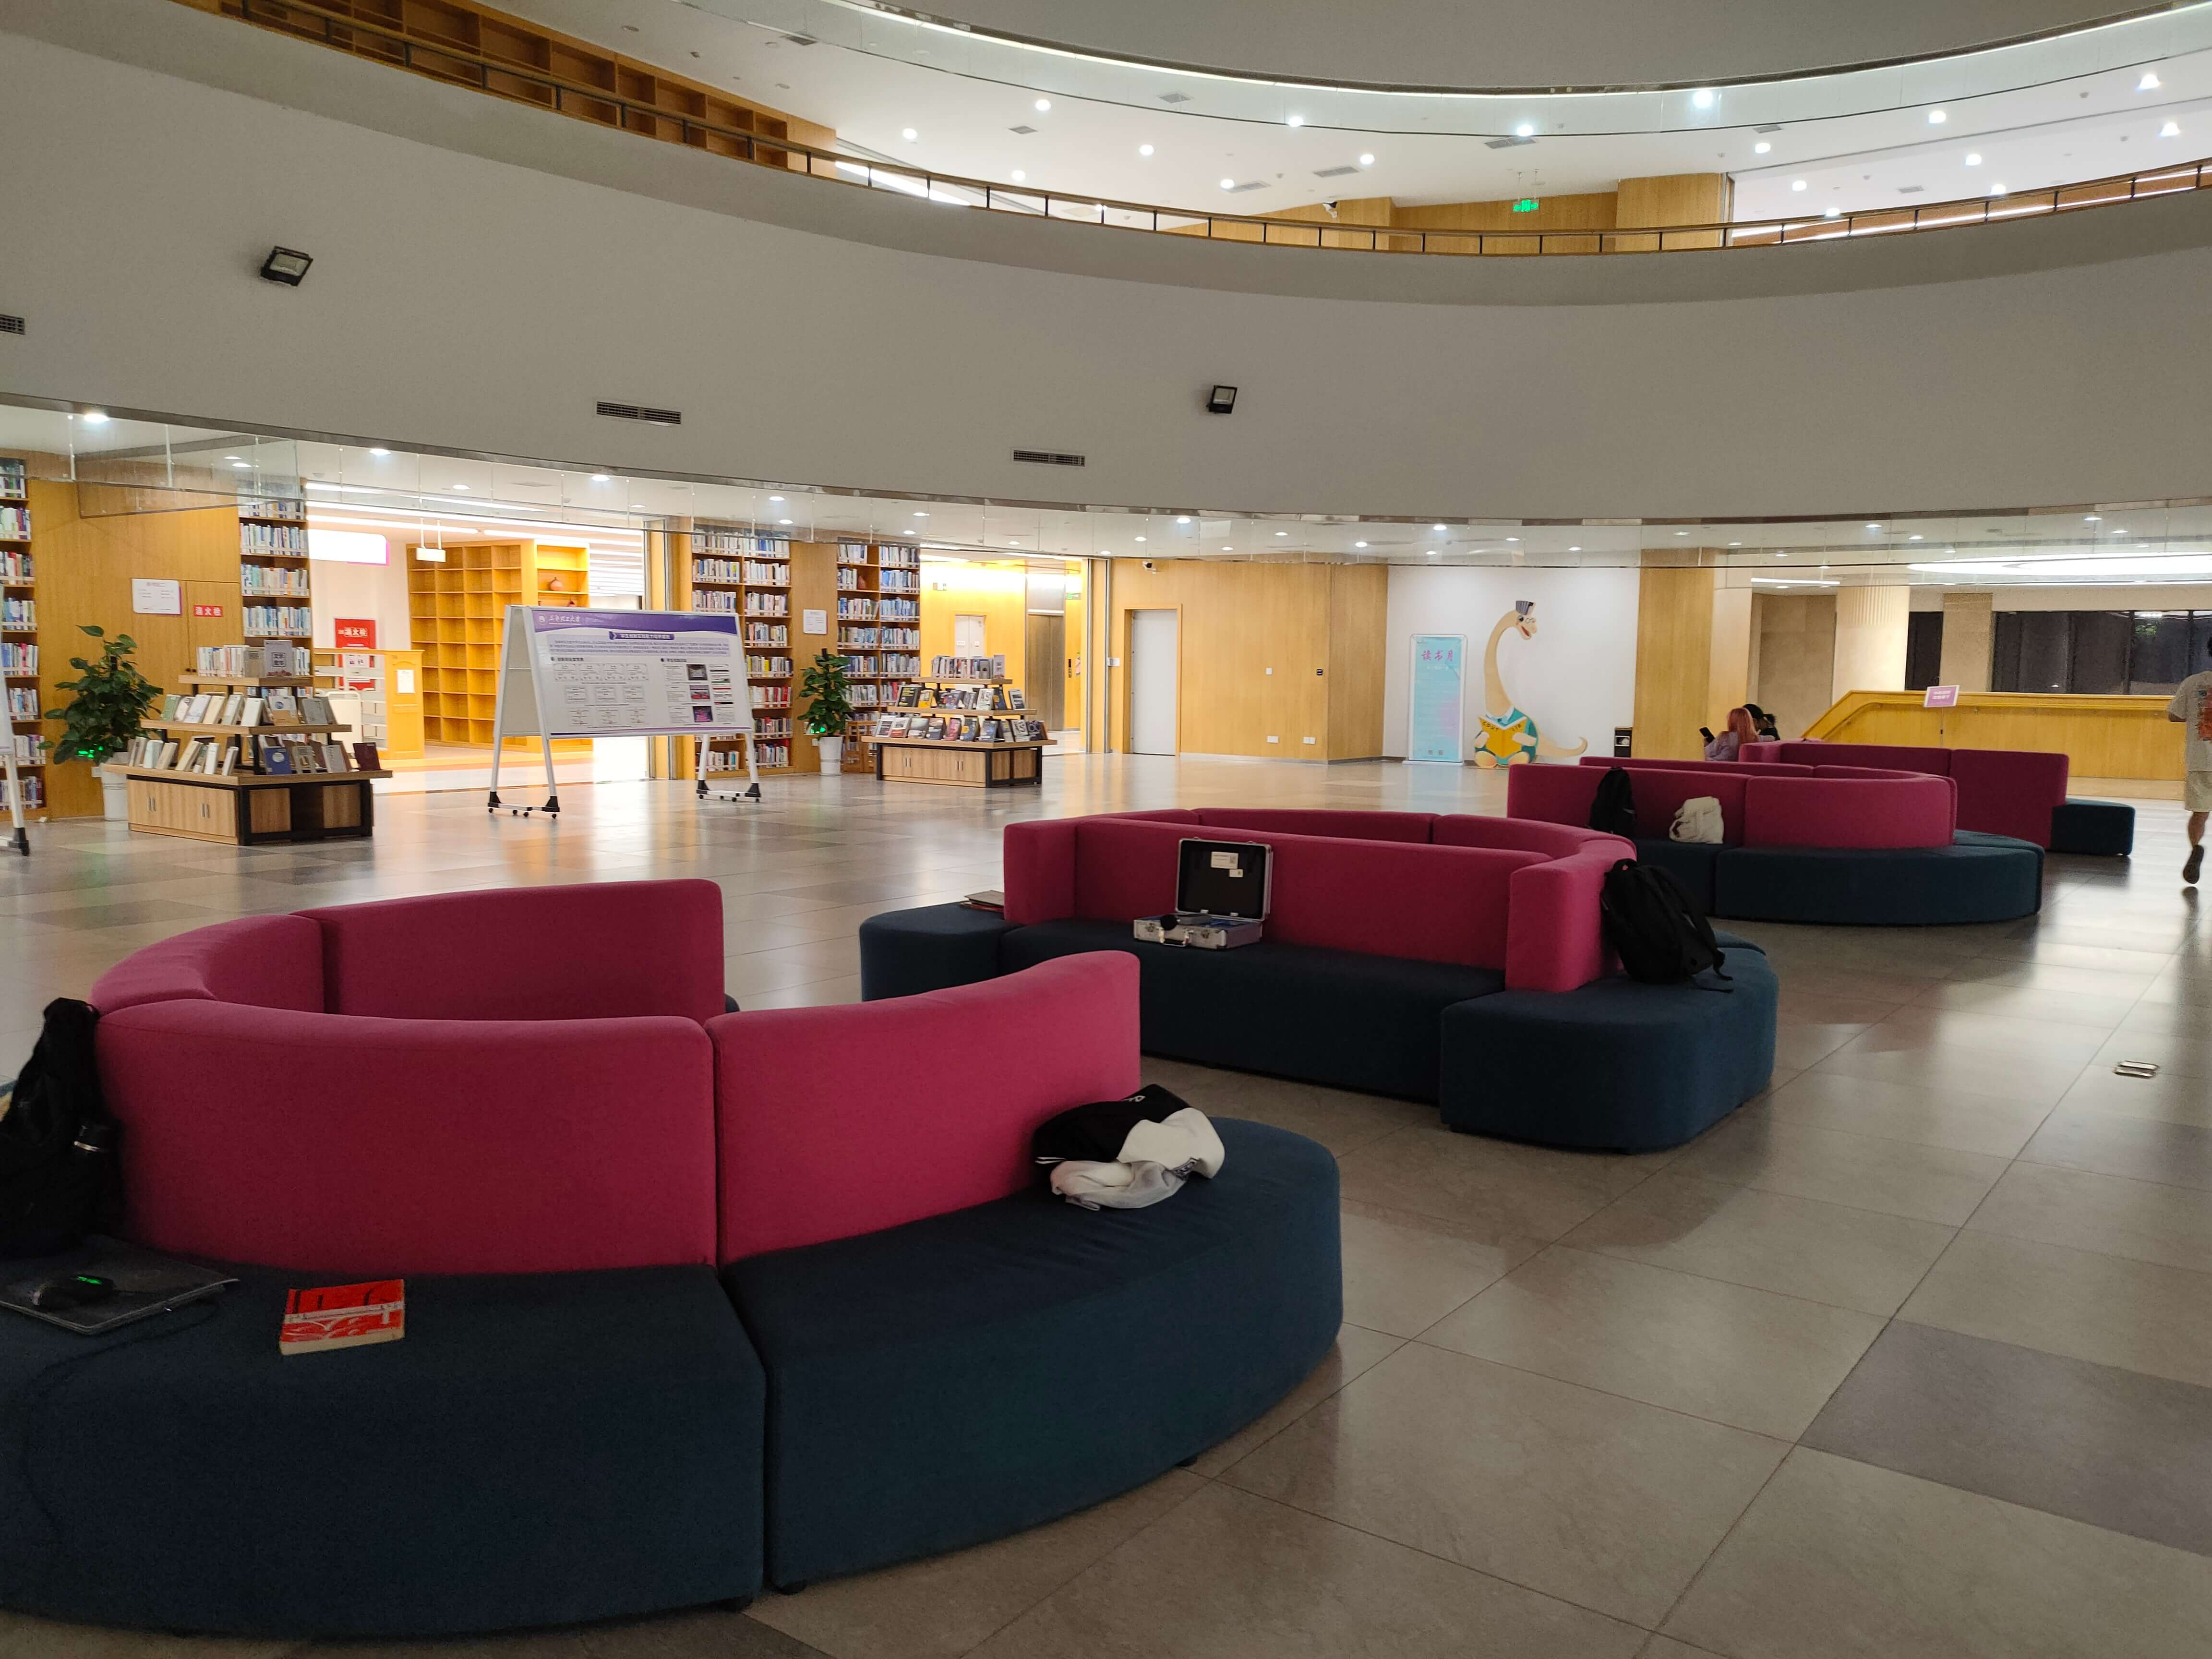
\includegraphics[width=\textwidth]{figures/Monitoring_point_-_center_on_the_second_floor_of_the_library.jpg}
        \caption{图书馆二楼中心}
    \end{subfigure}
    \hfill
    \begin{subfigure}[htb]{0.48\textwidth}
        \centering
        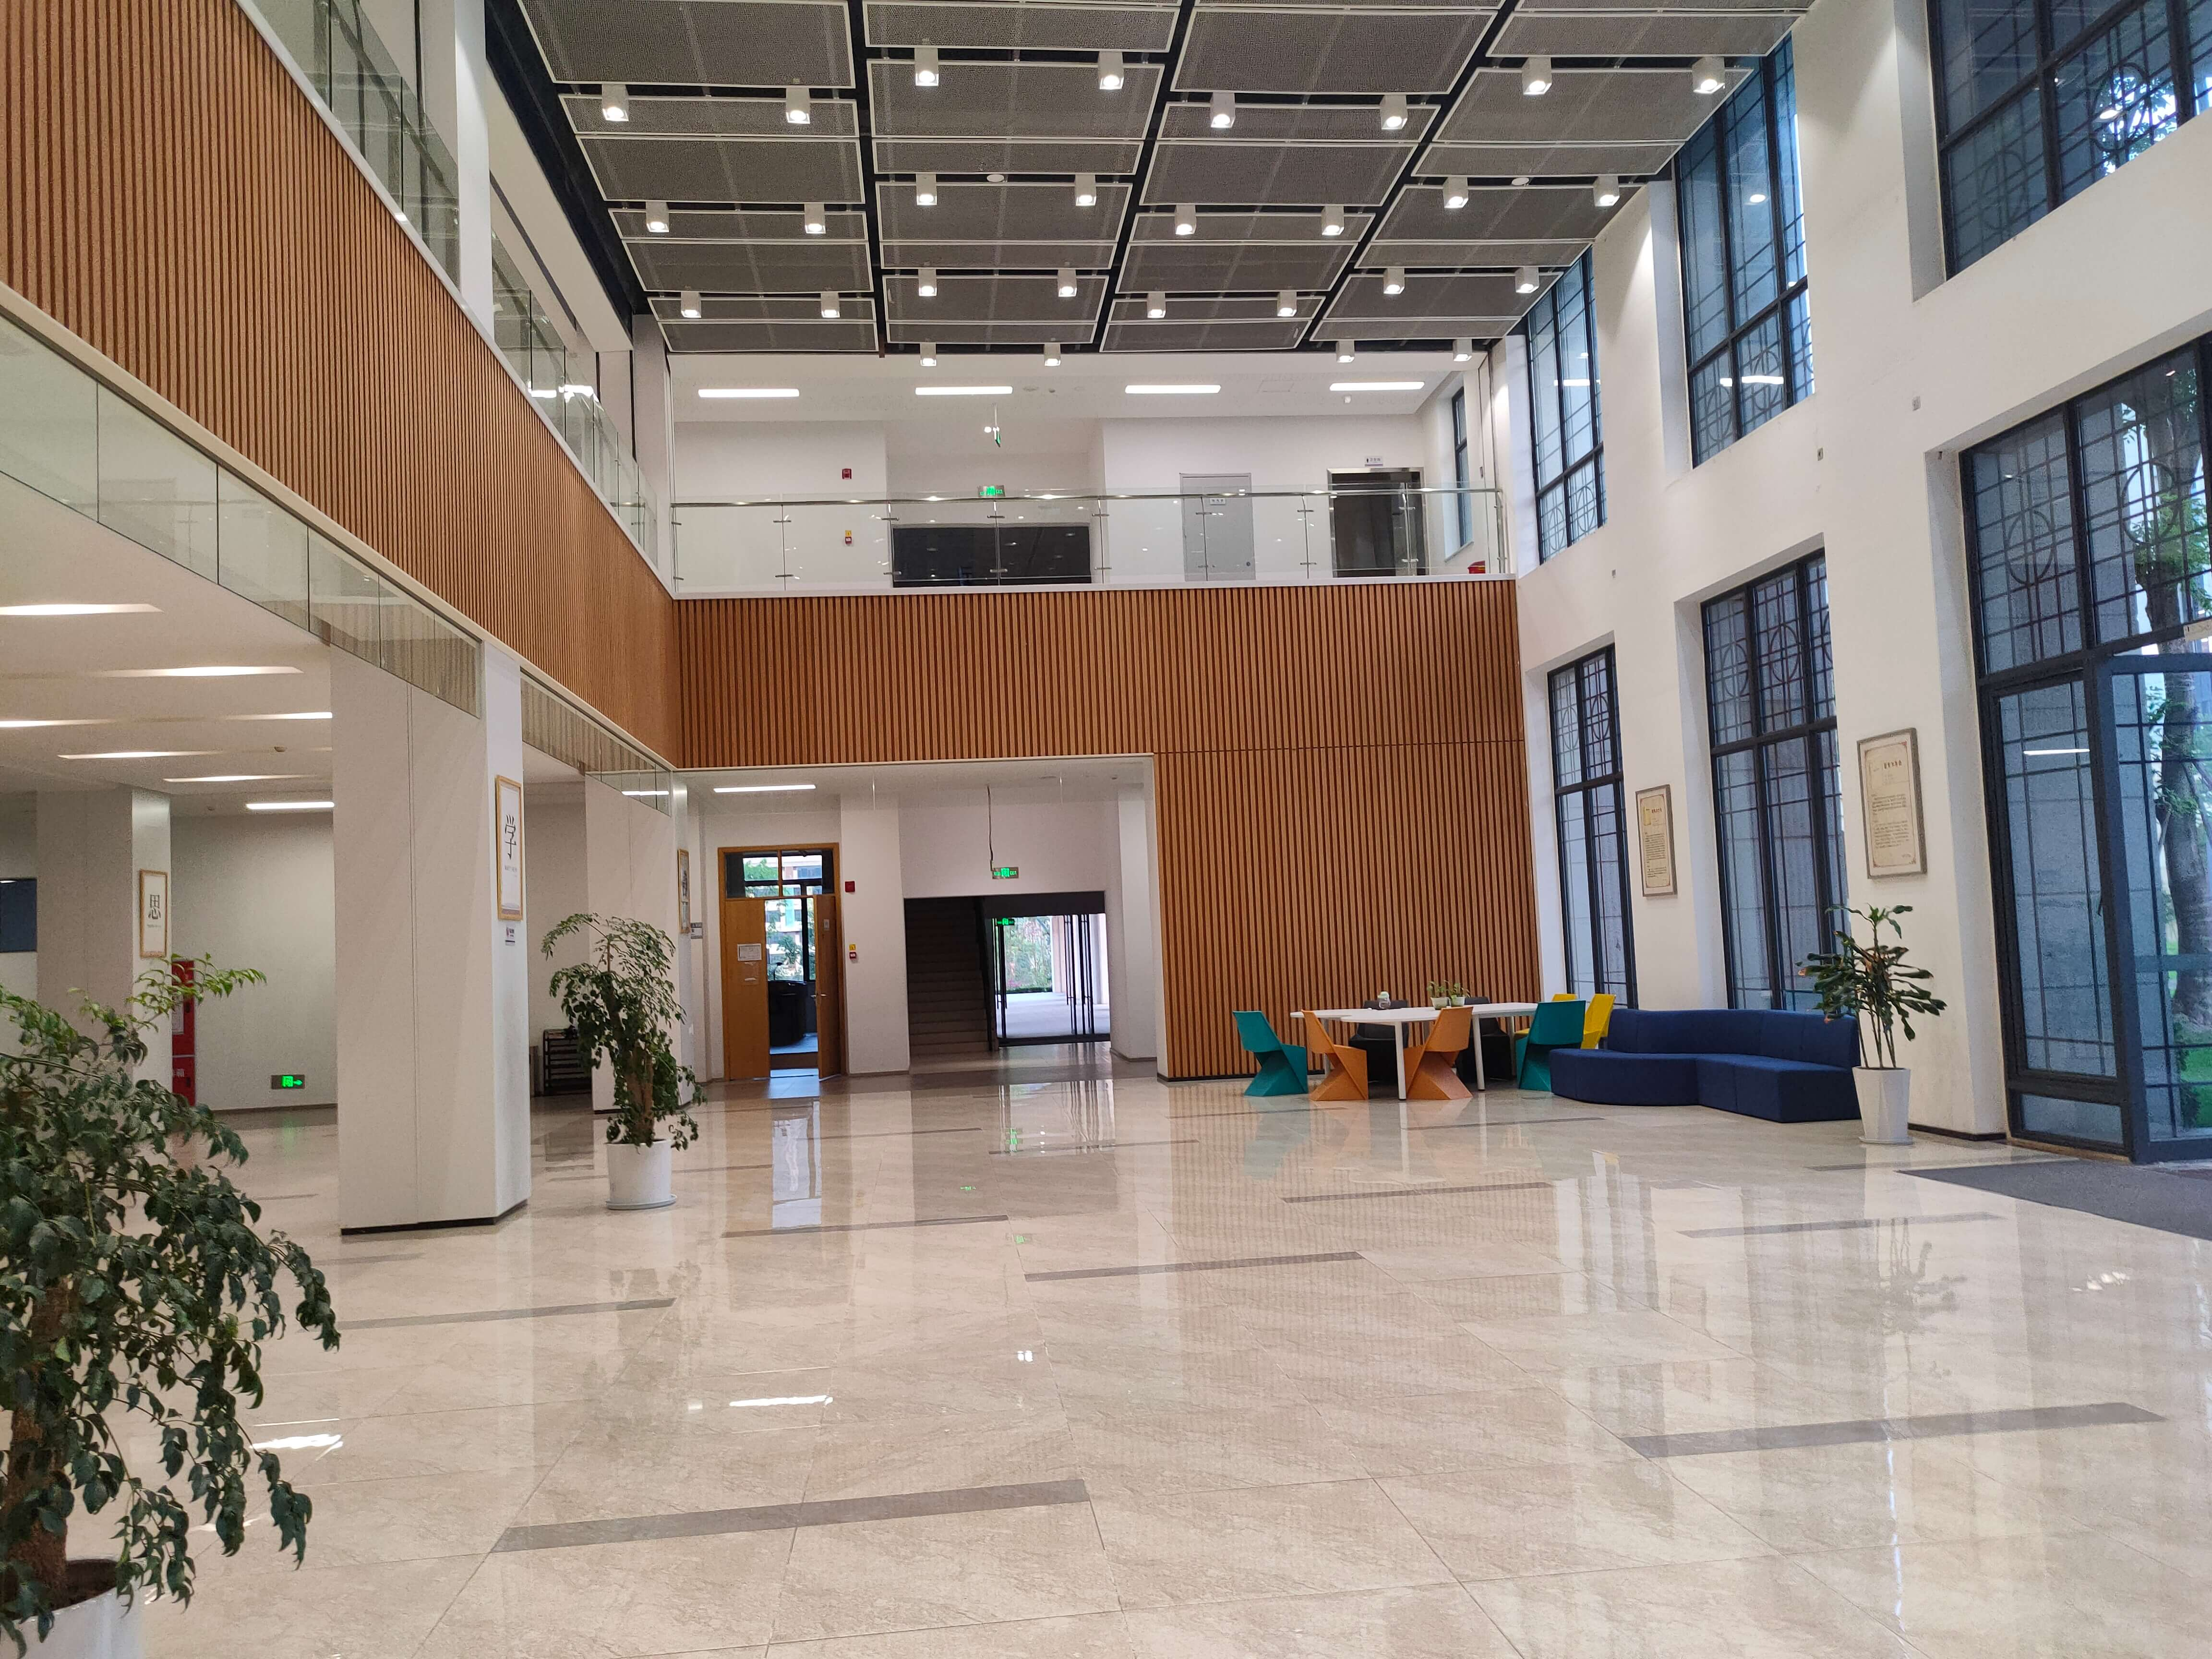
\includegraphics[width=\textwidth]{figures/Monitoring_point_-_the_first_floor_of_the_teaching_building.jpg}
        \caption{教学楼甲一楼}
    \end{subfigure}
    \hfill
    \begin{subfigure}[htb]{0.48\textwidth}
        \centering
        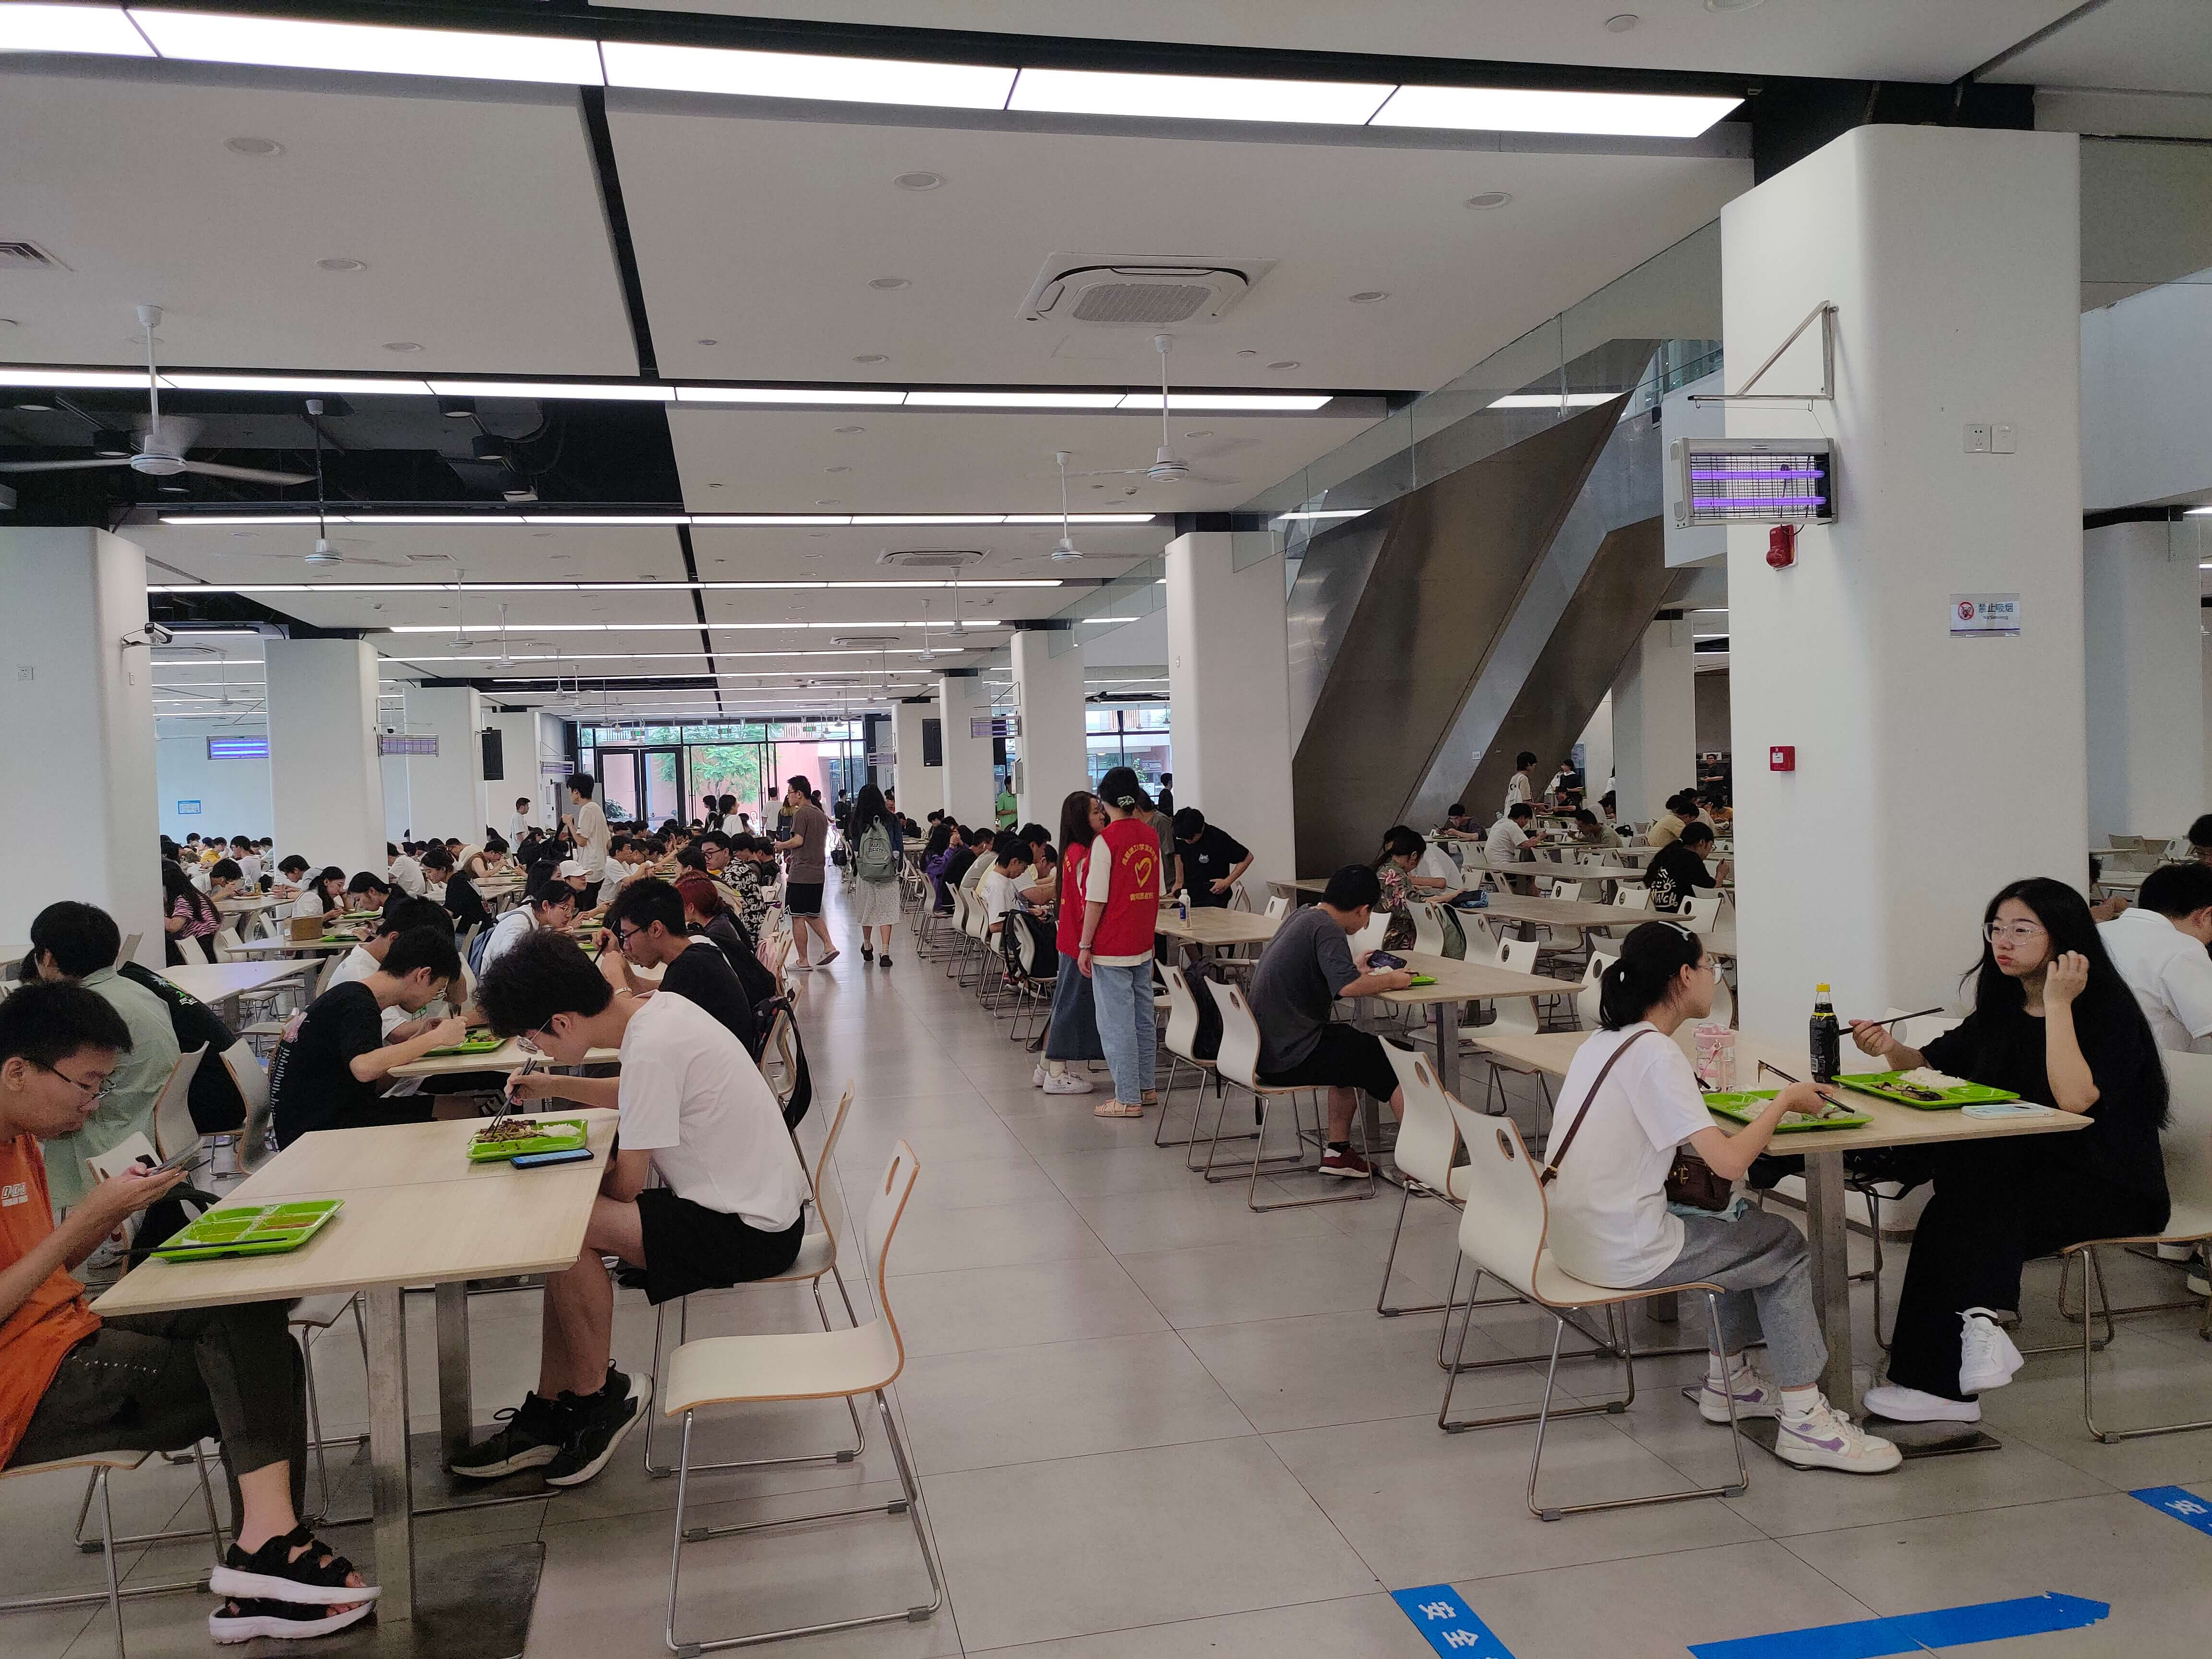
\includegraphics[width=\textwidth]{figures/Monitoring_point_-_the_first_floor_of_the_canteen_of_the_first_phase.jpg}
        \caption{一期食堂一楼}
    \end{subfigure}
    \caption{声环境监测点实时图}
    \label{fig:Sound_environment_monitoring_points}
\end{figure}


\subsubsection{监测项目说明}
\paragraph{$\bullet$ 监测时段}~{}\par
分别测定昼间和夜间的等效A声级,连续监测2天,昼、夜间各一次。

\begin{sidewaystable}[p]
    \centering
    \caption{声环境监测数据}
    \resizebox{\textwidth}{!}{
    \begin{tabular}{|c|c|c|c|c|c|c|c|c|c|c|c|c|c|c|c|}
    \multicolumn{16}{r}{单位:dB(A)} \\
    \hline
    \textbf{地点} & \textbf{时间} & \textbf{监测日期} & \textbf{风向} & \textbf{风速km/h} & \textbf{天气} & \textbf{Leq} & \textbf{SEL} & \textbf{Lmax} & \textbf{Lmin} & \textbf{L5} & \textbf{L10} & \textbf{L50} & \textbf{L90} & \textbf{L95} & \textbf{SD} \\
    \hline
    \multirow{4}*{教学楼甲一楼} & \multirow{2}*{$9:00-10:00$} & 2023/6/7 & 东北    & 2     & 晴     & 54.1  & 89.7  & 79.0  & 33.2  & 58.8  & 53.8  & 41.2  & 36.8  & 35.8  & 7.1  \\
    \cline{3-16}          &       & 2023/6/8 & 东北    & 6     & 小雨    & 51.9  & 87.5  & 80.1  & 32.8  & 56.0  & 50.2  & 38.8  & 34.8  & 34.4  & 6.7  \\
    \cline{2-16}          & \multirow{2}*{$19:30-20:30$} & 2023/6/6 & 西     & 4     & 晴     & 50.2  & 85.8  & 80.7  & 31.4  & 45.6  & 42.0  & 37.0  & 34.6  & 33.8  & 4.3  \\
    \cline{3-16}          &       & 2023/6/7 & 北     & 4     & 晴     & 52.6  & 88.2  & 79.1  & 33.6  & 55.6  & 51.4  & 43.0  & 37.2  & 36.4  & 6.1  \\
    \hline
    \multirow{4}*{体育馆二楼篮球场} & \multirow{2}*{$10:30-11:30$} & 2023/6/7 & 东     & 2     & 晴     & 70.4  & 106.0  & 96.8  & 53.5  & 74.2  & 72.8  & 68.6  & 64.2  & 62.8  & 3.5  \\
    \cline{3-16}          &       & 2023/6/8 & 东北    & 6     & 小雨转阴  & 69.8  & 105.4  & 88.8  & 56.3  & 73.0  & 72.2  & 69.2  & 66.0  & 65.0  & 2.4  \\
    \cline{2-16}          & \multirow{2}*{$20:00-21:00$} & 2023/6/6 & 西北    & 4     & 晴     & 68.8  & 104.4  & 89.8  & 51.8  & 73.4  & 71.4  & 66.4  & 61.8  & 60.6  & 3.9  \\
    \cline{3-16}          &       & 2023/6/7 & 北     & 4     & 晴     & 65.7  & 101.3  & 88.1  & 44.0  & 70.8  & 69.0  & 63.2  & 57.8  & 56.2  & 4.4  \\
    \hline
    \multirow{4}*{图书馆二楼中心} & \multirow{2}*{$9:30-10:30$} & 2023/6/7 & 东     & 2     & 晴     & 42.8  & 78.4  & 59.0    & 29.9  & 48.8  & 46.6  & 38.8  & 33.6  & 32.6  & 4.9 \\
    \cline{3-16}          &       & 2023/6/8 & 东北    & 6     & 小雨    & 43.8  & 79.4  & 73.7  & 28.9  & 48.2  & 45.8  & 38.2  & 32.8  & 31.8  & 5.0 \\
    \cline{2-16}          & \multirow{2}*{$21:00-22:00$} & 2023/6/6 & 北     & 5     & 晴     & 49.2  & 84.8  & 80.1  & 45.2  & 51.0    & 49.0  & 47.4  & 46.8  & 46.6  & 1.6 \\
    \cline{3-16}          &       & 2023/6/7 & 北     & 4     & 晴     & 43.6  & 79.2  & 66.0  & 30.1  & 50.6  & 44.6  & 37.2  & 33.4  & 32.6  & 5.1 \\
    \hline
    \multirow{4}*{一期食堂一楼} & \multirow{2}*{$11:30-12:30$} & 2023/6/7 & 东南    & 2     & 晴     & 68.8  & 104.4 & 82.1  & 63.1  & 71.6  & 70.8  & 68.2  & 66.0  & 65.4  & 1.9 \\
    \cline{3-16}          &       & 2023/6/8 & 东北    & 10    & 小雨转阴  & 68.6  & 104.2 & 83.7  & 63.0  & 71.4  & 70.6  & 68.0  & 65.8  & 65.2  & 1.8 \\
    \cline{2-16}          & \multirow{2}*{$22:00-23:00$} & 2023/6/6 & 北     & 3     & 晴     & 52.3  & 87.2  & 89.5  & 41.8  & 53.6  & 51.2  & 46.8  & 44.4  & 44.0  & 3.4 \\
    \cline{3-16}          &       & 2023/6/7 & 北     & 4     & 晴     & 50.2  & 85.8  & 69.0  & 39.7  & 54.6  & 53.2  & 48.6  & 43.2  & 42.2  & 3.8 \\
    \hline
    \end{tabular}}
    \label{tab:Summary of monitoring records}
\end{sidewaystable}


\paragraph{$\bullet$ 监测方法及数据统计}~{}\par
使用AWA5688多功能声级计,按标准规范执行,即按《社会生活环境噪声排放标准》(GB 22337-2008)进行测量。监测各测点处的连续等效A声级。


\paragraph{$\bullet$ 数据处理}~{}\par
按国家标准方法和推荐方法进行,提供$\mathrm{L_{Aeq}}$值。
环境噪声评价量,等效声级 $\mathrm{L_{eq}}$ 计算公式:
\begin{equation} \label{eq:how to get Leq}
	\mathrm{L_{eq}} = 10\lg{\dfrac{1}{N}\sum^N_{i=1}10^{0.1L_i}}
\end{equation}
式中:$L_i$——第 $i$ 次读取的A声级;\newline
\phantom{式中:}$N$——取样总数。

将数据按顺序排列找出 $\mathrm{L_{5}}$、$\mathrm{L_{10}}$、$\mathrm{L_{50}}$、$\mathrm{L_{90}}$、$\mathrm{L_{95}}$,
并计算出噪声标准差 SD :
\begin{equation}
    \text{{SD}} = \sqrt{\frac{1}{N}\sum_{i=1}^{N}(X_i - \bar{X})^2}
\end{equation}
其中,$N$表示样本的数量; \\
\phantom{其中,}$X_i$表示第$i$个样本值; \\
\phantom{其中,}$\bar{X}$表示样本均值。

因为监测的时间为1小时 $T=3600$ s,所以可以计算出暴露声压级:
\begin{align}
    \text{SEL} &= \mathrm{L_{eq}} + 10\lg{(T)} \\
    &= \mathrm{L_{eq}} + 10\lg{(3600)} \notag
\end{align}

点声源的几何发散衰减计算公式:
\begin{align} \label{eq:Geometric divergence attenuation calculation of point sound sources}
    % A_{div} = 10\lg{\dfrac{1}{4\pi r^2}} \\
    A_{div} = 20\lg{\dfrac{r}{r_0}}
\end{align}
式中:$A_{div}$——几何发散引起的衰减,dB;\\
\phantom{式中:}$r$——预测点距声源的距离;\\
\phantom{式中:}$r_0$——参考位置距声源的距离。

 

\subsubsection{监测评价相关标准}
% \begin{itemize}
%     \item 《声环境质量标准》( GB 3096-2008)
%     \item 《社会生活环境噪声排放标准》( GB 22337-2008)
%     \item 《环境影响评价技术导则——声环境》( HJ 2.2-2018)
% \end{itemize}

根据《声环境质量标准》( GB 3096-2008)声环境功能区分类标准,按照区域的使用功能特点和环境质量要求,将声环境功能区划分为五种类型:
\begin{enumerate}[label={\arabic*类声环境功能区:},align=left, leftmargin=*]
    \setcounter{enumi}{-1}
    \item 指康复疗养区等特别需要安静的区域。
    \item 指以居民住宅、医疗卫生、文化教育、科研设计、行政办公为主要功能,需要保持安静的区域。
    \item 指以商业金融、集市贸易为主要功能,或者居住、商业、工混杂,需要维护住宅安静的区域。
    \item 指以工业生产、仓储物流为主要功能,需要防止工业噪声对周围环境产生严重影响的区域。
    \item 指交通干线两侧一定区域之内,需要防止交通噪声对周围环境产生严重影响的区域,包括4a类和4b类两种类型。4a类为高速公路、一级公路、二级公路、城市快速路、城市主干路、城市次干路、城市轨道交通(地面段)、内河航道两侧区域;4b类为铁路干线两侧区域。
\end{enumerate}

\begin{table}[H]
    \centering
    \caption{环境噪声限值\cite{GB3096-2008}}
    \begin{tabular}{|c|c|c|c|}
        \multicolumn{4}{r}{单位:dB(A)} \\
        \hline
        \multicolumn{2}{|c|}{\multirow{2}*{\hspace{2em}声环境功能区类别\hspace{2em}}} & \multicolumn{2}{c|}{时段} \\
        \cline{3-4}    \multicolumn{2}{|c|}{} & \hspace{2em}昼间\hspace{2em}    & \hspace{2em}夜间\hspace{2em} \\
        \hline
        \multicolumn{2}{|c|}{0类} & 50    & 40 \\
        \hline
        \multicolumn{2}{|c|}{1类} & 55    & 45 \\
        \hline
        \multicolumn{2}{|c|}{2类} & 60    & 50 \\
        \hline
        \multicolumn{2}{|c|}{3类} & 65    & 55 \\
        \hline
        \multirow{2}*{\hspace{2em}4类\hspace{2em}} & 4a类   & 70    & 55 \\
        \cline{2-4} & 4b类   & 70    & 60 \\
        \hline
    \end{tabular}
    \label{tab:Ambient noise limits}
\end{table}

由于我们选择的监测点位于校园的文化教育区域,因此根据声环境功能区的分类,这些点属于1类声环境功能区。所以环境噪声限值为:
$\text{昼间}\leqslant 55 \;\mathrm{dB(A)}$,$\text{夜间}\leqslant 45 \;\mathrm{dB(A)}$。


\subsection{报告主体部分}

\subsubsection{数据加工}

因为声环境监测方案选定了一个地点选定昼夜两次,连续两天(见表 \ref{tab:Summary of monitoring records})。所以在进行相同时段分析的时候,根据公式 \ref{eq:how to get Leq} 计算出同时段等效声级如下表所示:

\begin{table}[H]
    \centering
    \caption{同时段等效声级}
    \begin{tabular}{|c|c|c|c|}
    \hline
    \textbf{地点} & \textbf{昼夜} & \textbf{计算过程} & \textbf{同时段等效声级 dB(A)} \\\hline
    \multirow{2}*{教学楼甲一楼} & 昼  & $10\lg{(10^{5.41}+10^{5.19})/2}$  & 53.14  \\\cline{2-4}
            & 夜  & $10\lg{(10^{5.02}+10^{5.26})/2}$   & 51.56  \\\hline
    \multirow{2}*{体育馆二楼篮球场} & 昼  & $10\lg{(10^{7.04}+10^{6.98})/2}$   & 70.11  \\\cline{2-4}
            & 夜  & $10\lg{(10^{6.88}+10^{6.57})/2}$   & 67.52  \\\hline
    \multirow{2}*{图书馆二楼中心} & 昼  & $10\lg{(10^{4.28}+10^{4.38})/2}$   & 43.33  \\\cline{2-4}
            & 夜  & $10\lg{(10^{4.92}+10^{4.36})/2}$   & 47.25  \\\hline
    \multirow{2}*{一期食堂一楼} & 昼  & $10\lg{(10^{6.88}+10^{6.86})/2}$   & 68.70  \\\cline{2-4}
            & 夜  & $10\lg{(10^{5.23}+10^{5.02})/2}$   & 51.38  \\\hline
    \end{tabular}
    \label{tab:Equivalent sound levels in the same segment}
\end{table}
  
这几天平均昼间温度为 25℃,相对湿度为 80\%;夜间温度为 25℃,相对湿度为 80\%。则可以通过EIAN和Sufer两个软件进行衰减预测,绘制不同点源分布的衰减等声线图。


\subsubsection{EIAN 2.0 操作步骤}
\begin{enumerate}
    \item 文件 $\rightarrow $ 背景图形文件 $\rightarrow $ 插入图形 $\rightarrow $ 定义两个点
    \begin{enumerate}[label=\arabic*)]
        \item 在奥维互动地图中找到合适的俯视全景图,想办法导出 .jpg 格式的图片文件,然后插入背景图片;
        \begin{figure}[H]
            \centering
            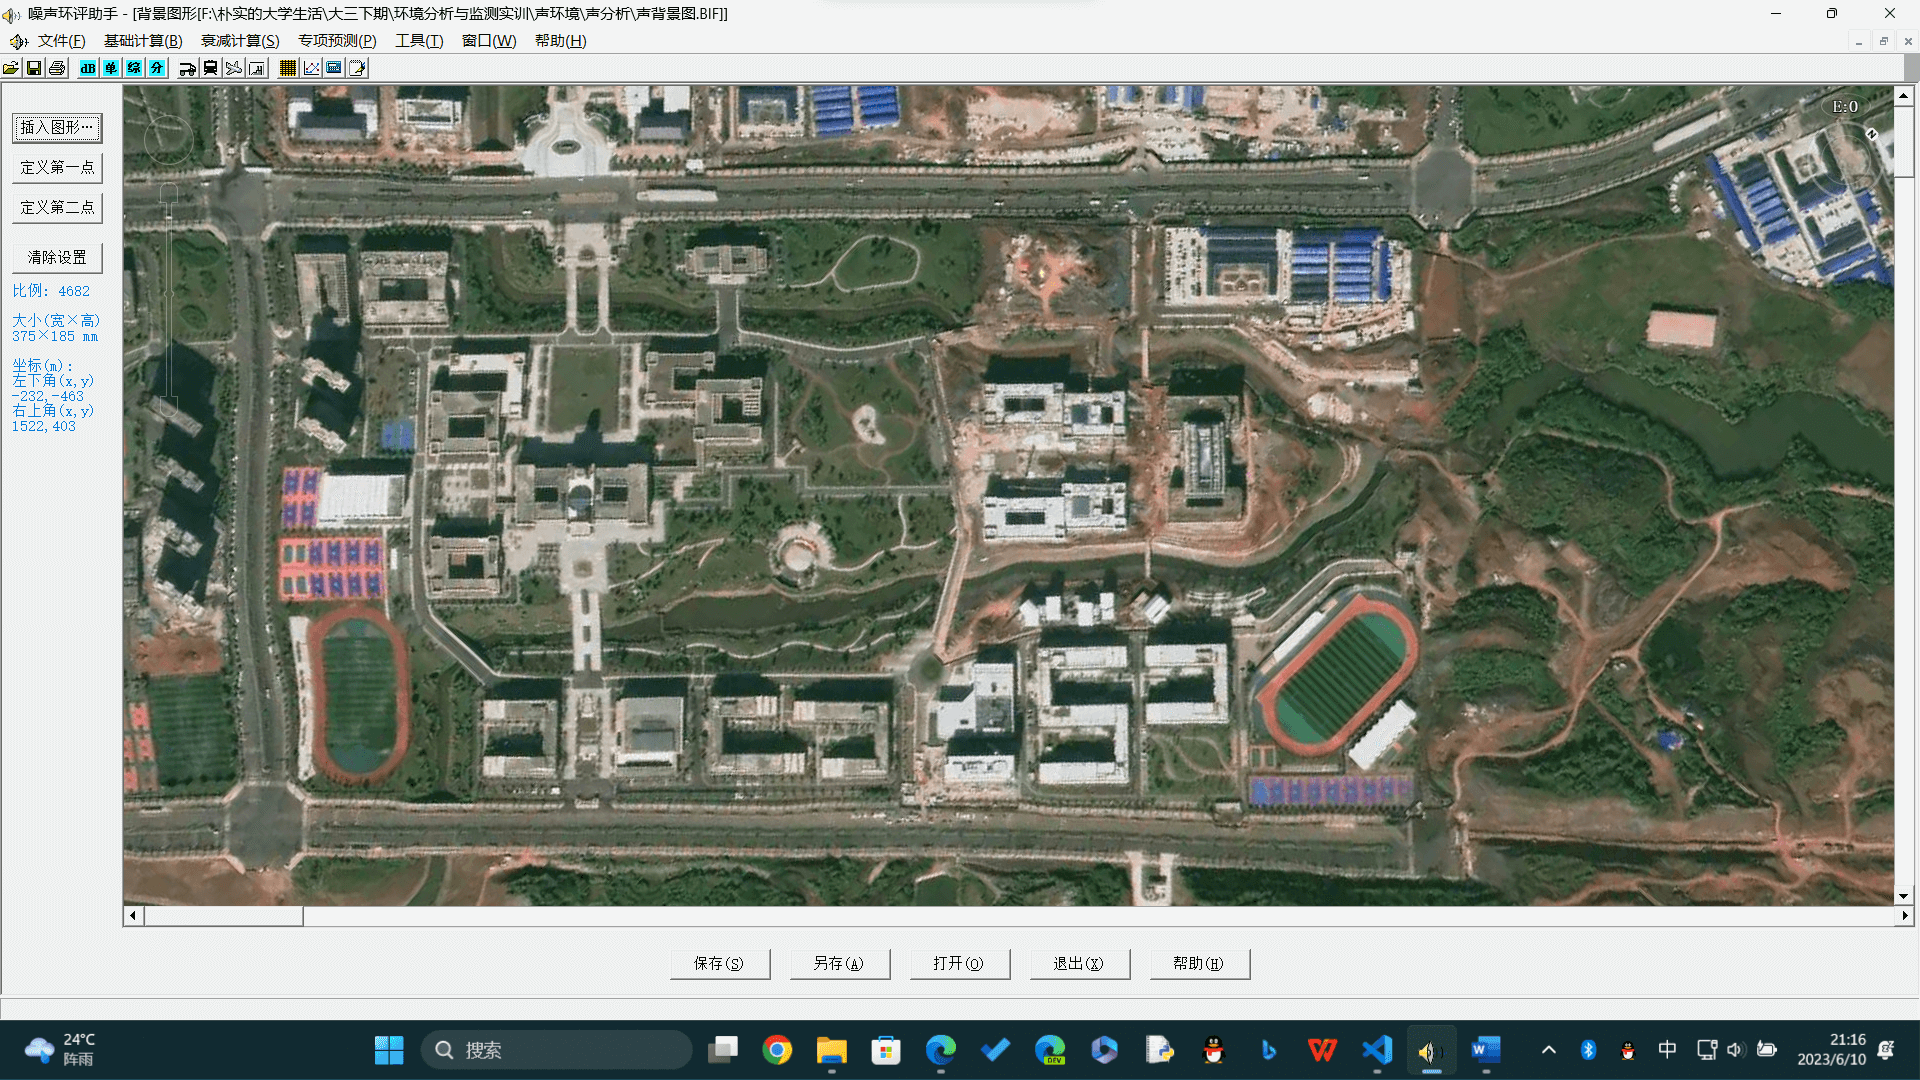
\includegraphics[width=0.8\textwidth]{figures/acoustic_step1.png}
            \caption{插入背景图形文件}
        \end{figure}

        \item 定义第一点:体育馆二楼篮球场 $(0,0)$ ;
        \item 定义第二点:图书馆二楼中心 $(220,0)$ ;
        \item 设置实际距离为 228 m。
    \end{enumerate}
    
    \item 衰减计算 $\rightarrow $ 噪声衰减分布计算 $\rightarrow $ 声源属性
    \begin{enumerate}[label=\arabic*)]
        \item 设置一般属性(名称、坐标、声源离地面高度);
        \begin{itemize}
            \item 体育馆二楼篮球场:坐标 $(0,0)$,高度为 5 m
            \item 图书馆二楼中心:坐标 $(220,0)$,高度为 1 m
            \item 教学楼甲一楼:坐标 $(339,84)$,高度为 1 m
            \item 一期食堂一楼:坐标 $(291,-242)$,高度为 1 m
        \end{itemize}
        \begin{figure}[H]
            \centering
            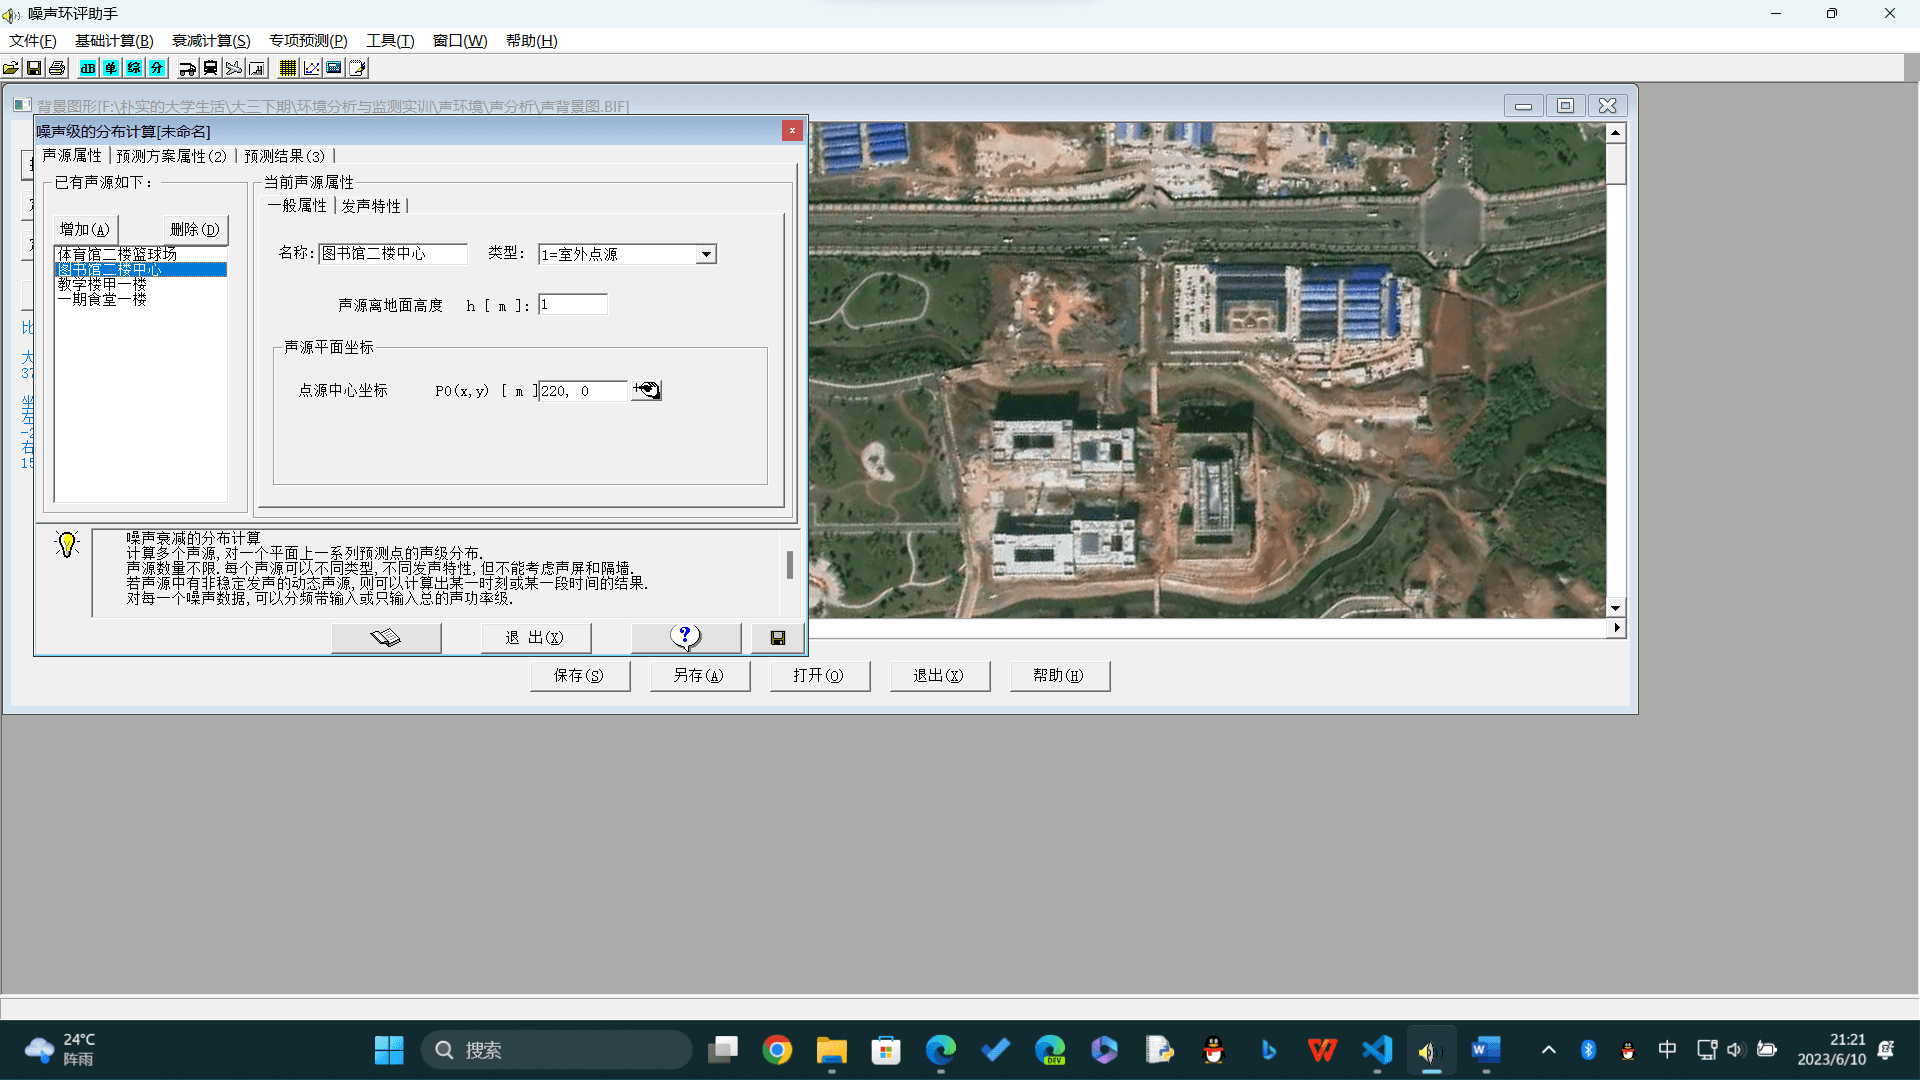
\includegraphics[width=0.8\textwidth]{figures/acoustic_step2-1.png}
            \caption{一般属性}
        \end{figure}

        \item 因为总声功率级为A计权,所以设置发声特性中总的声功率级的代表频率都为 1000 Hz。因此,只需要设置各噪声源总的声功率级(或A声功率级)。
        \begin{itemize}
            \item 体育馆二楼篮球场(昼/夜):70.11/67.52 dB(A)
            \item 图书馆二楼中心(昼/夜):43.33/47.25 dB(A)
            \item 教学楼甲一楼(昼/夜):53.14/51.56 dB(A)
            \item 一期食堂一楼(昼/夜):68.70/51.38 dB(A)
        \end{itemize}
        \begin{figure}[H]
            \centering
            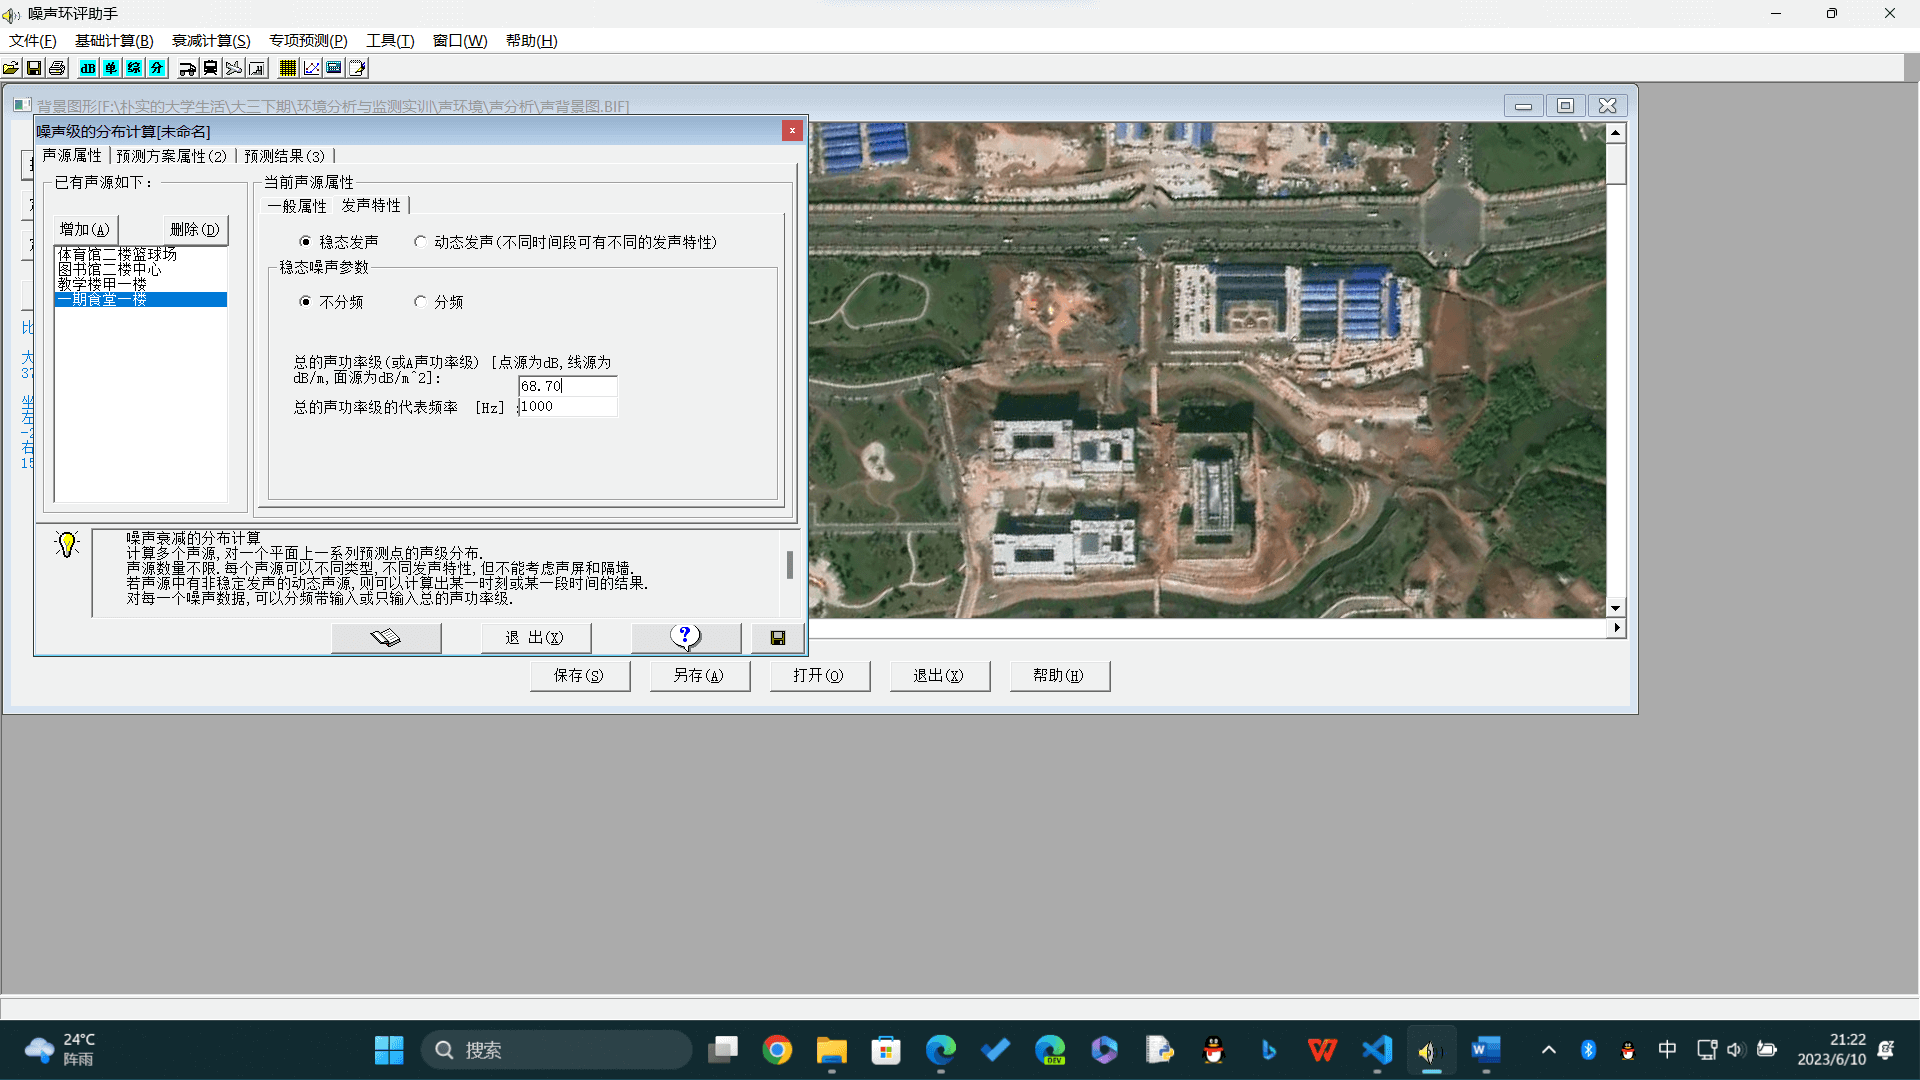
\includegraphics[width=0.8\textwidth]{figures/acoustic_step2-2.png}
            \caption{发声特性}
        \end{figure}
    \end{enumerate}
    
    \item 噪声衰减分布计算 $\rightarrow $ 预测方案属性
    \begin{enumerate}[label=\arabic*)]
        \item 选择“从背景图形上取得坐标”,然后画出来预测范围;
        \begin{figure}[H]
            \centering
            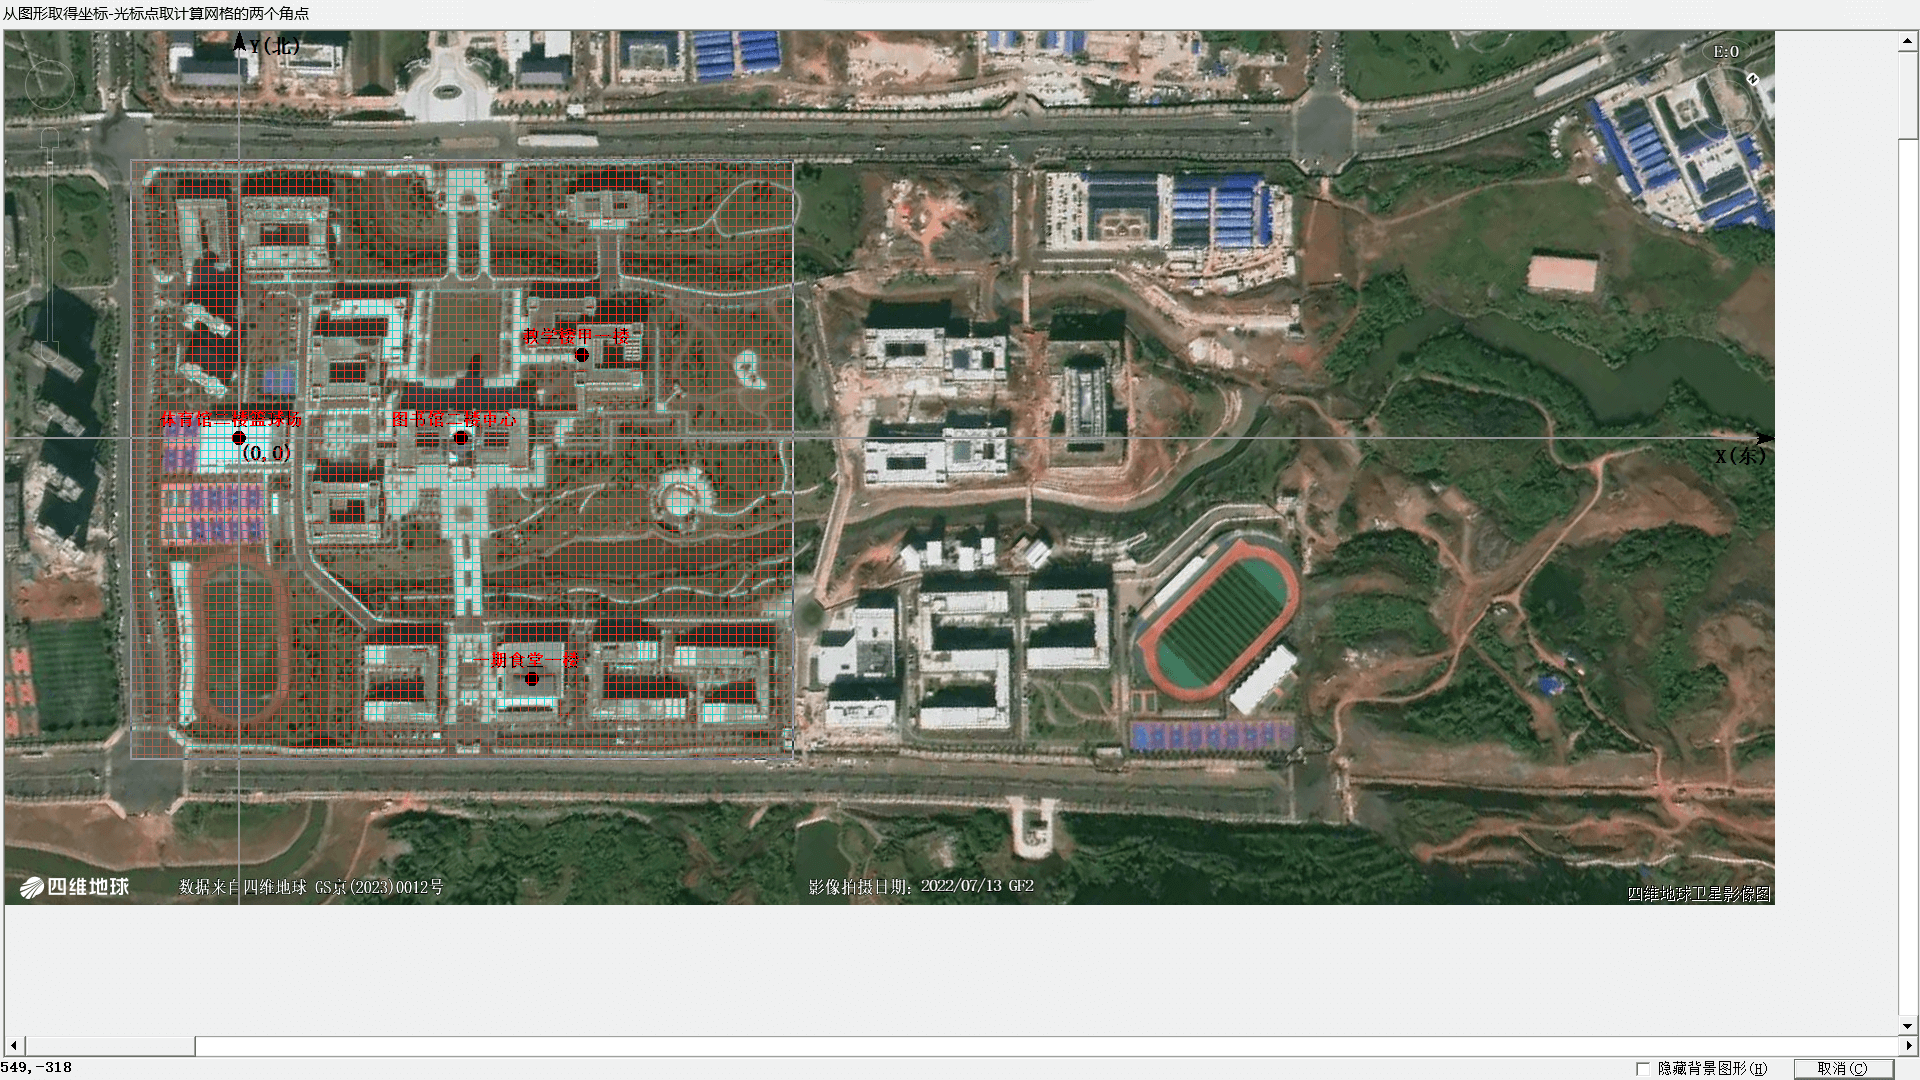
\includegraphics[width=0.8\textwidth]{figures/acoustic_step3-1.png}
            \caption{框选预测范围}
        \end{figure}

        \item 设置环境空气参数;
        \begin{itemize}
            \item 环境空气温度:25 ℃
            \item 空气相对湿度:80 \%
            \item 空气大气压:1 atm
        \end{itemize}
        \item 预测点X坐标与Y坐标的步长,默认值是100m,画出的图形为趋势图,这里调整为10m;
        \item 预测结果选项全部勾选。
        \begin{itemize}
            \item 考虚虑空气吸收的衰减量
            \item 考虑地面吸收的衰减量
        \end{itemize}
        \begin{figure}[H]
            \centering
            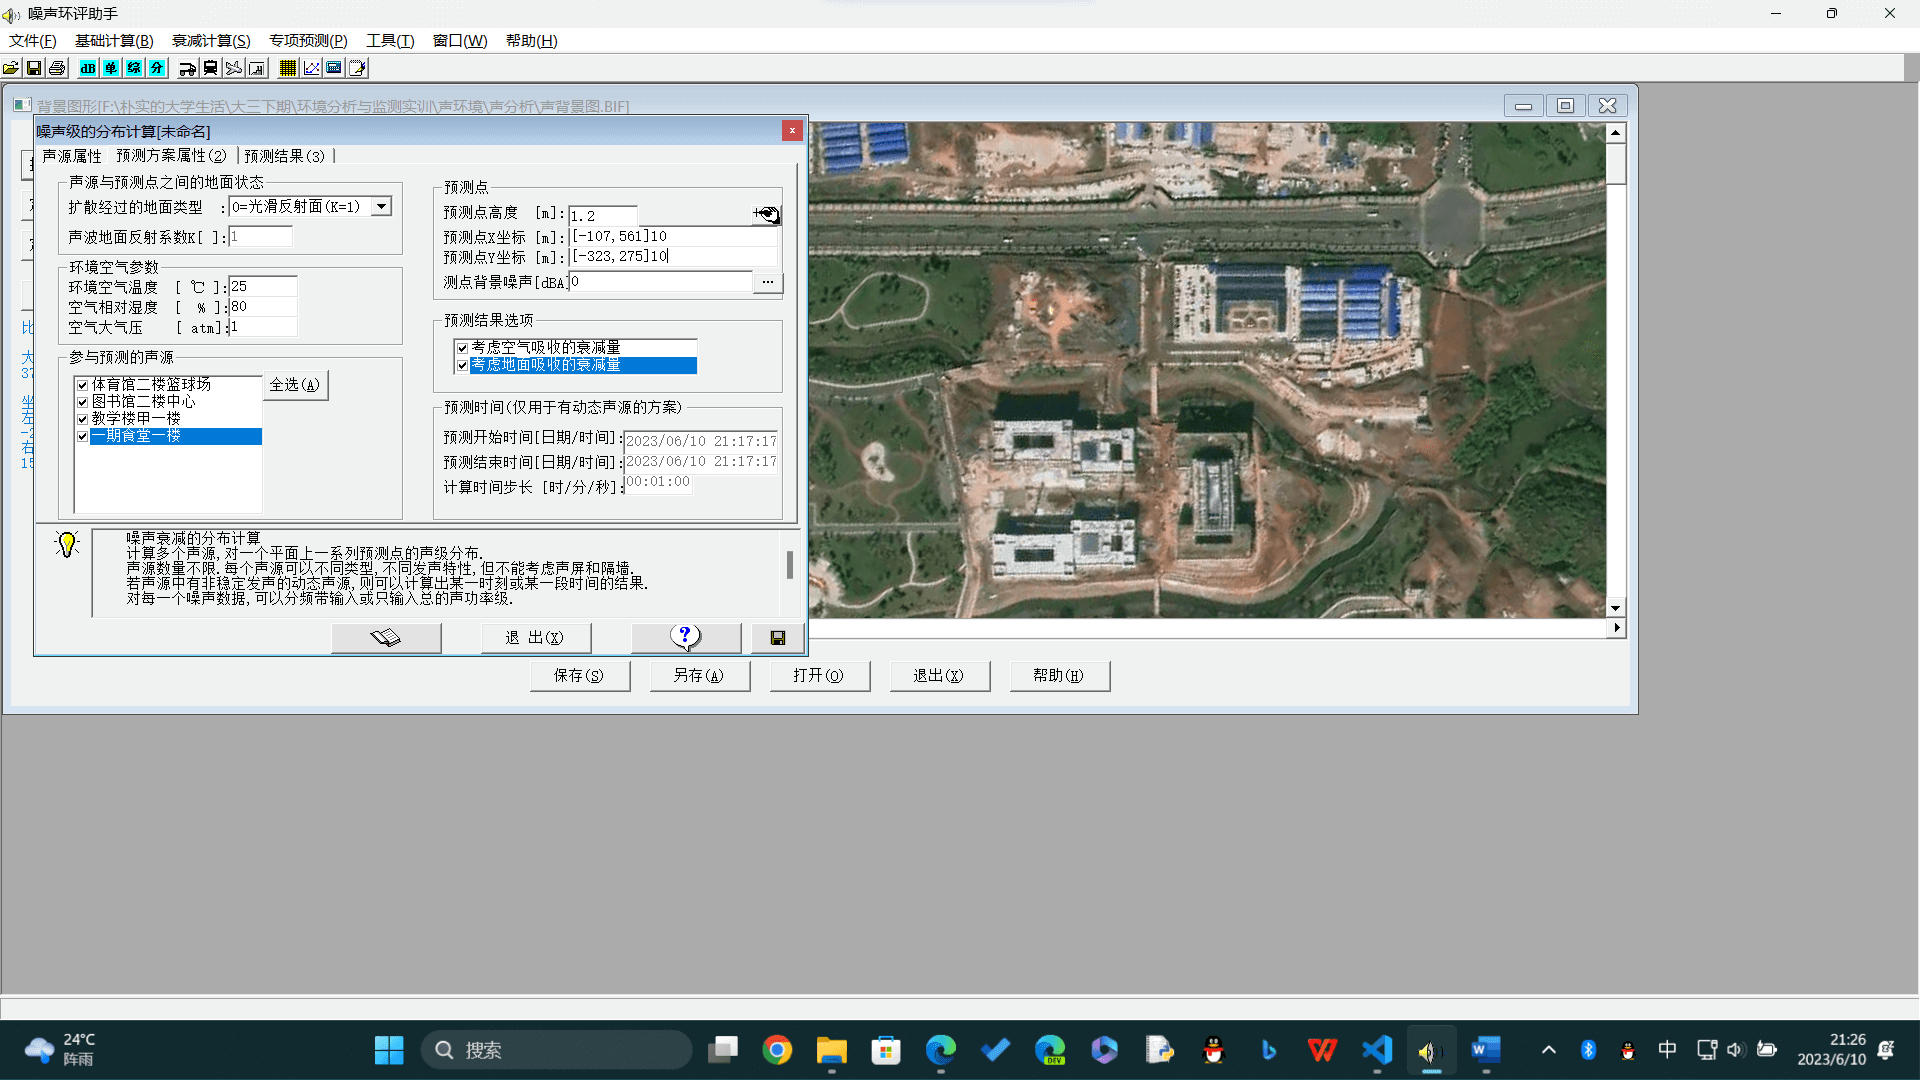
\includegraphics[width=0.8\textwidth]{figures/acoustic_step3-2.png}
            \caption{预测属性修改}
        \end{figure}
    \end{enumerate}

    \item 噪声衰减分布计算 $\rightarrow $ 预测结果 $\rightarrow $ 刷新结果
    \begin{figure}[H]
        \centering
        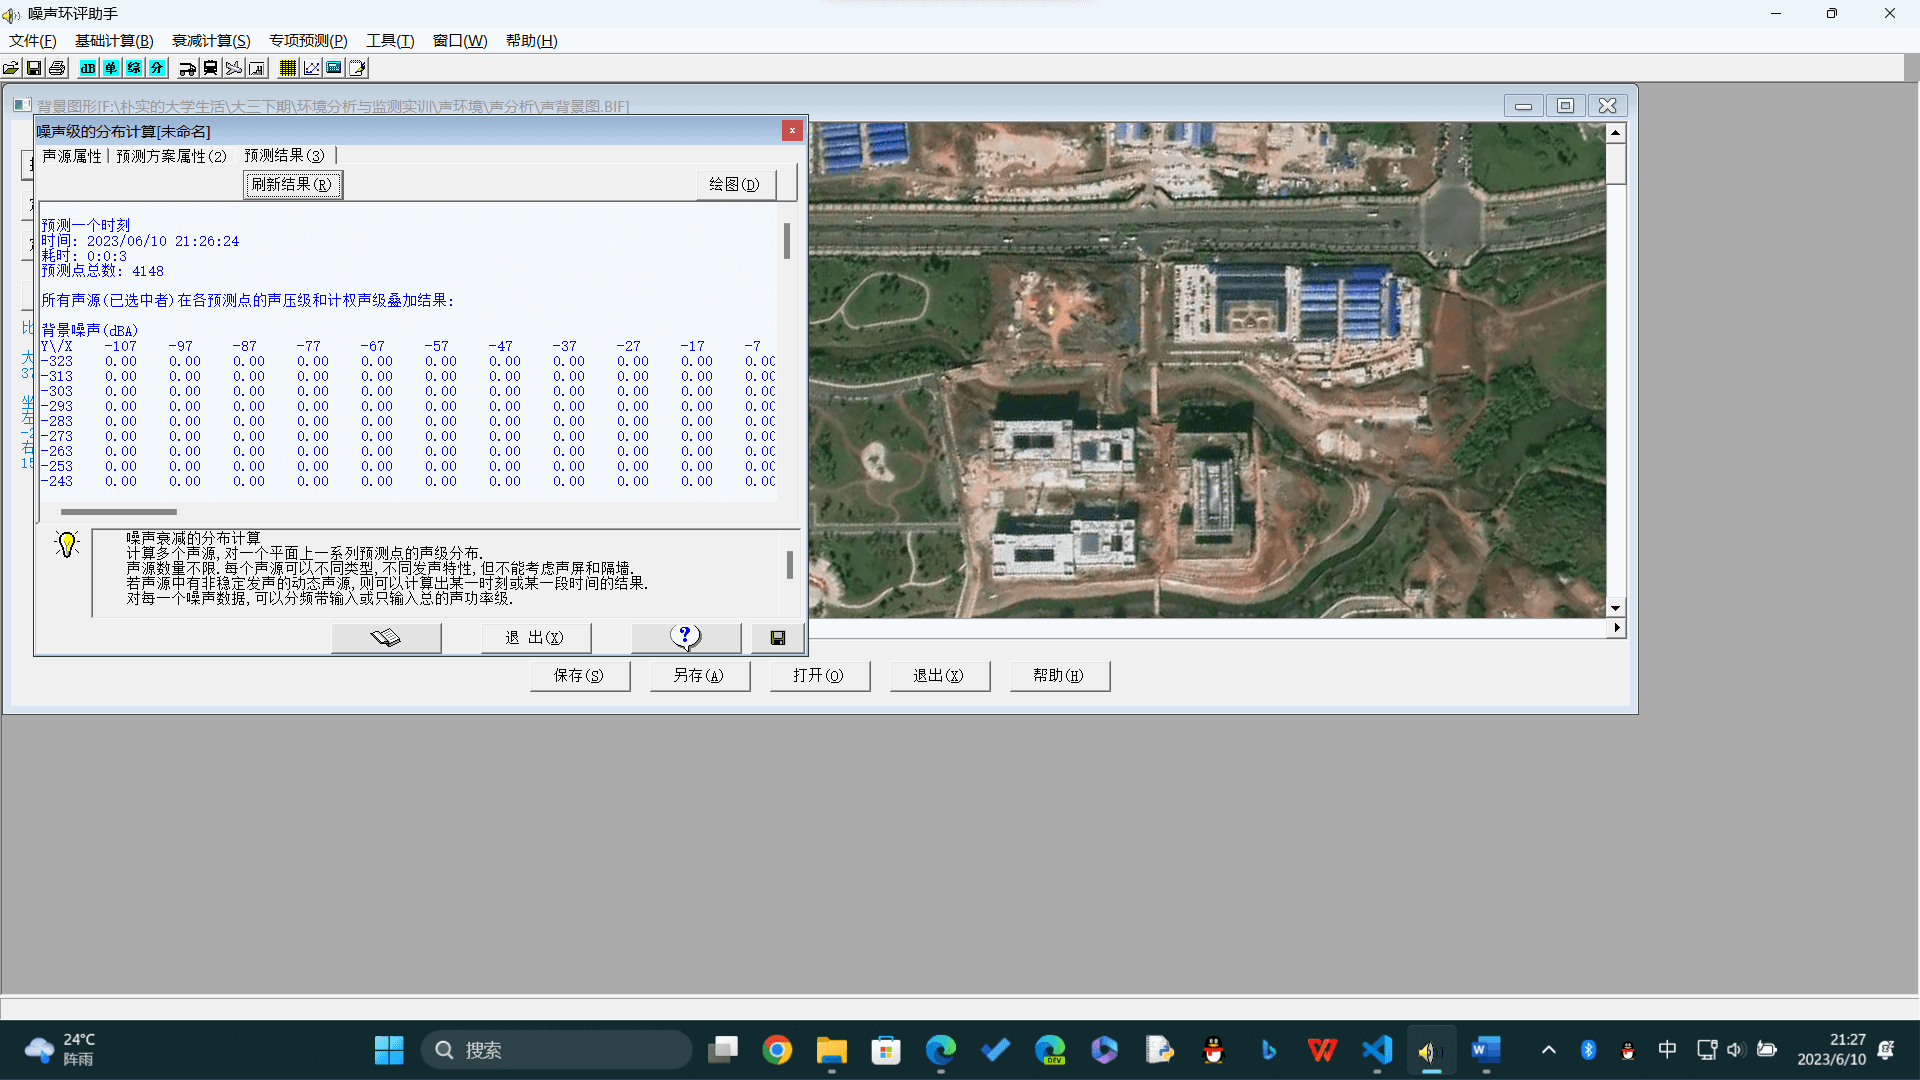
\includegraphics[width=0.8\textwidth]{figures/acoustic_step4.png}
        \caption{生成噪声衰减结果}
        \label{fig:Generate noise attenuation results}
    \end{figure}
    刷新得到的预测结果复制保存到.txt文件或者Excel文件中,为之后使用Sufer软件绘图提供噪声衰减数据。

    \item 预测结果 $\rightarrow $ 绘图 $\rightarrow $ A计权声级dB(A)
    % \begin{figure}[H]
    %     \centering
    %     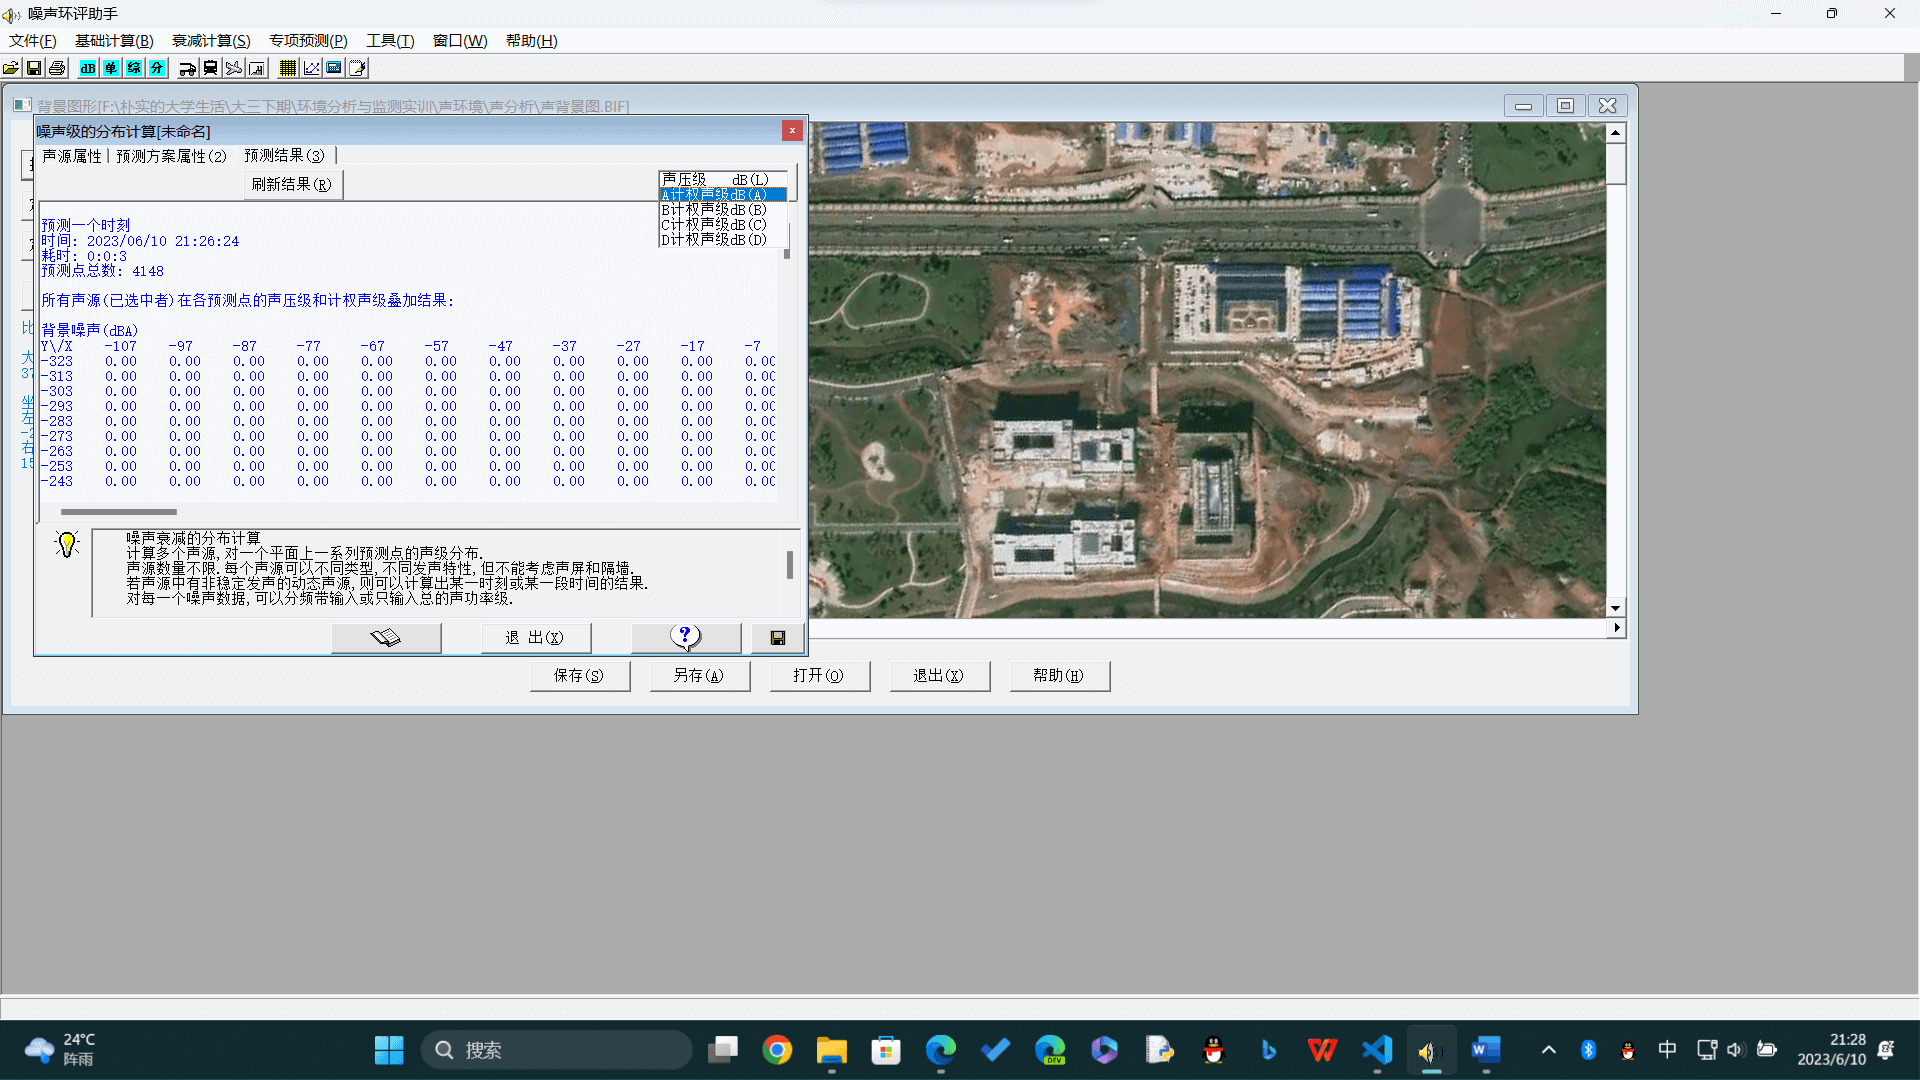
\includegraphics[width=0.8\textwidth]{figures/acoustic_step5.png}
    %     \caption{绘制A计权声级图}
    % \end{figure}

    \item 最后,生成昼夜两个时段的校园噪声衰减图:
    \begin{figure}[H]
        \centering
        \begin{subfigure}[h]{\textwidth}
            \centering
            % 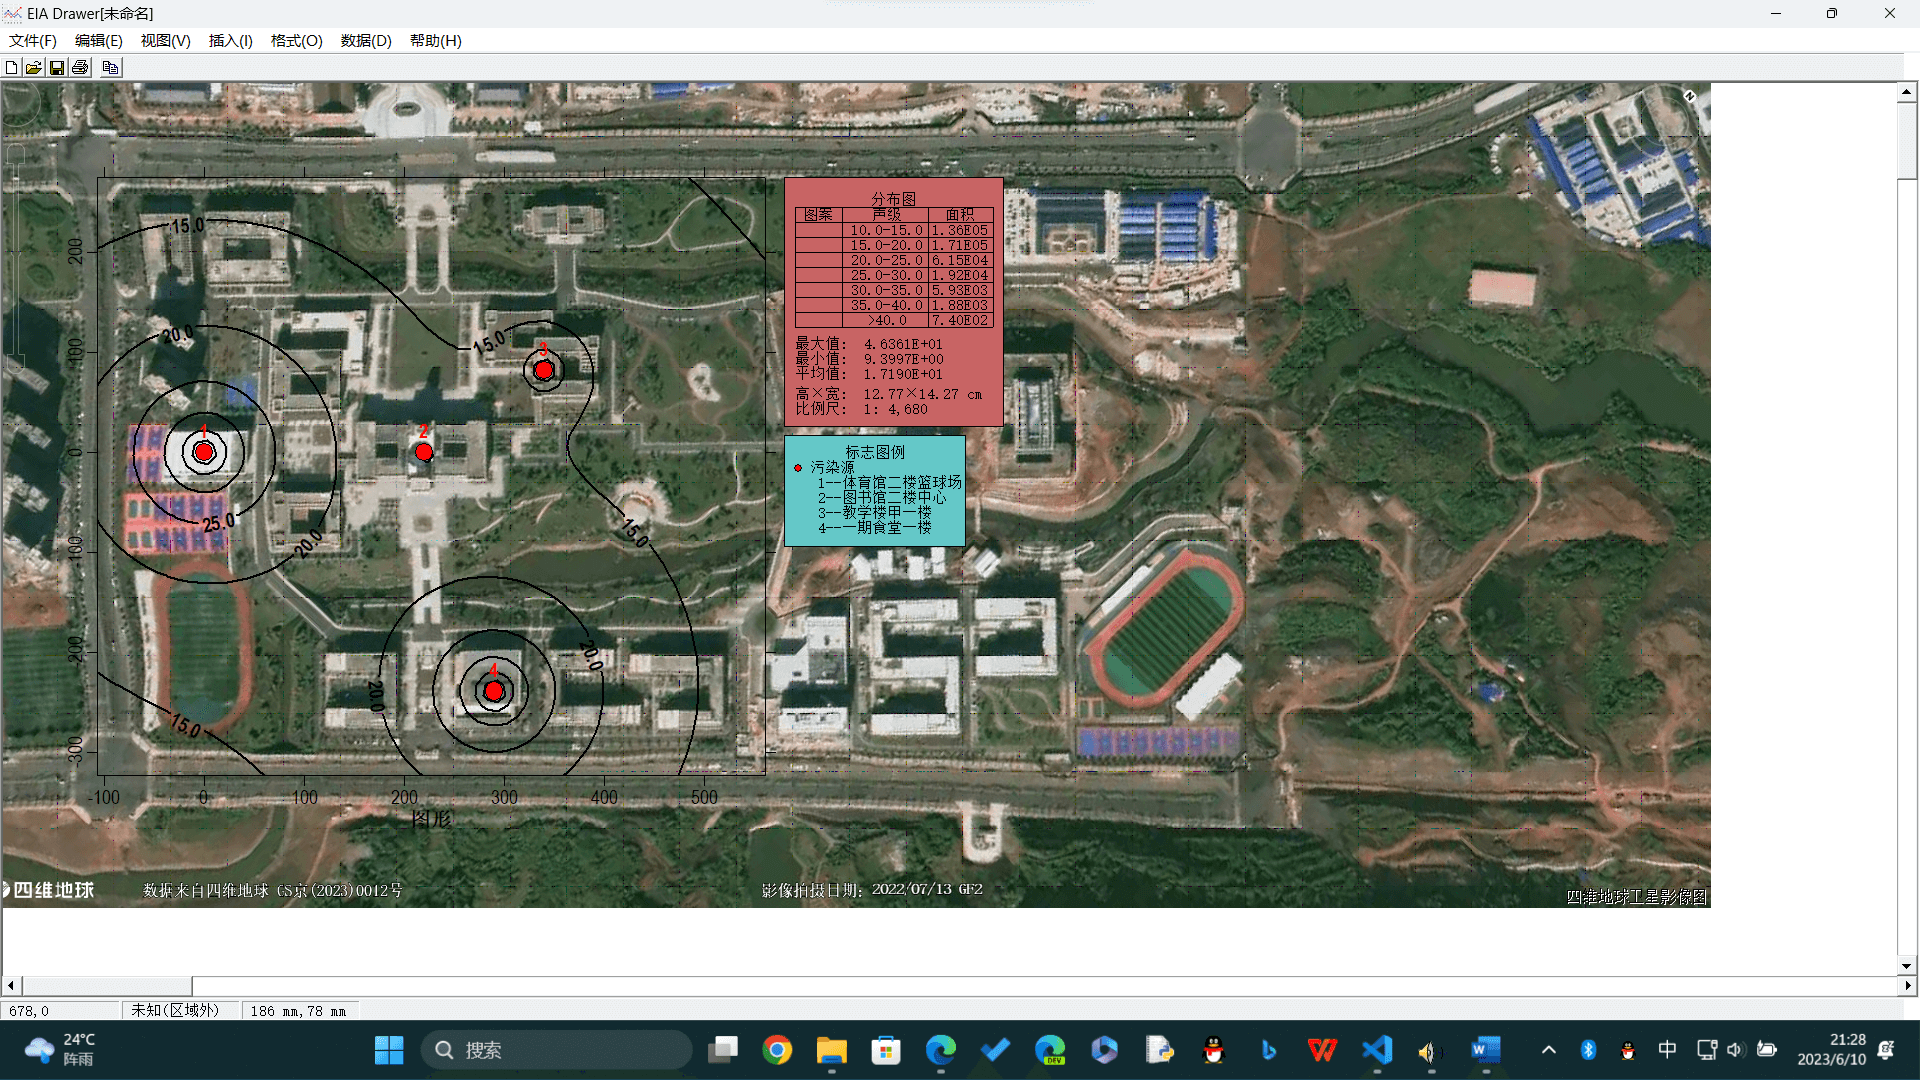
\includegraphics[width=0.8\textwidth]{figures/acoustic_step6-1.png}
            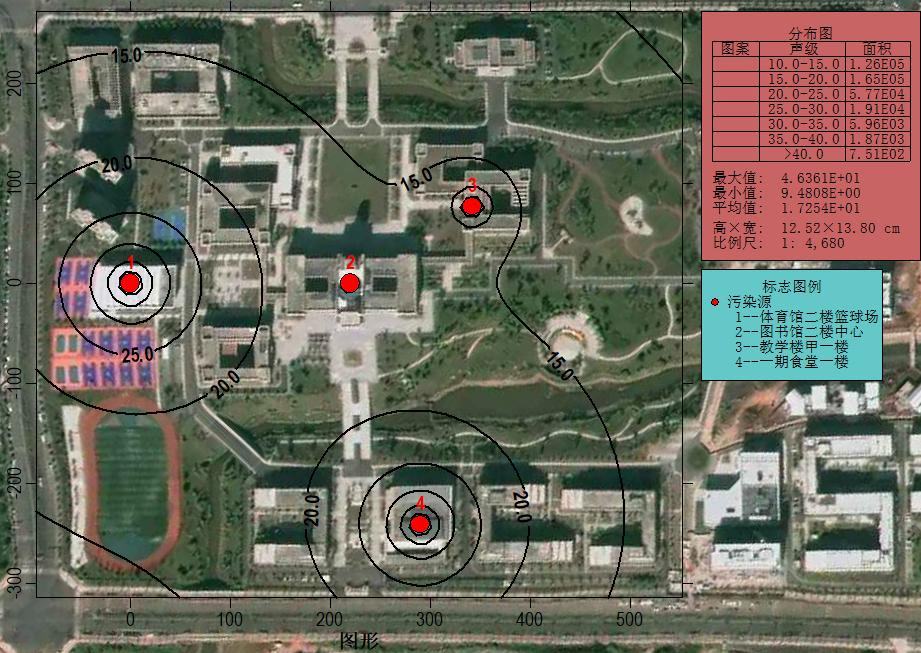
\includegraphics[width=0.8\textwidth]{figures/Campus noise attenuation plot-daytime.jpg}
            \caption{昼}
        \end{subfigure}
        \hfill
        \begin{subfigure}[h]{\textwidth}
            \centering
            % 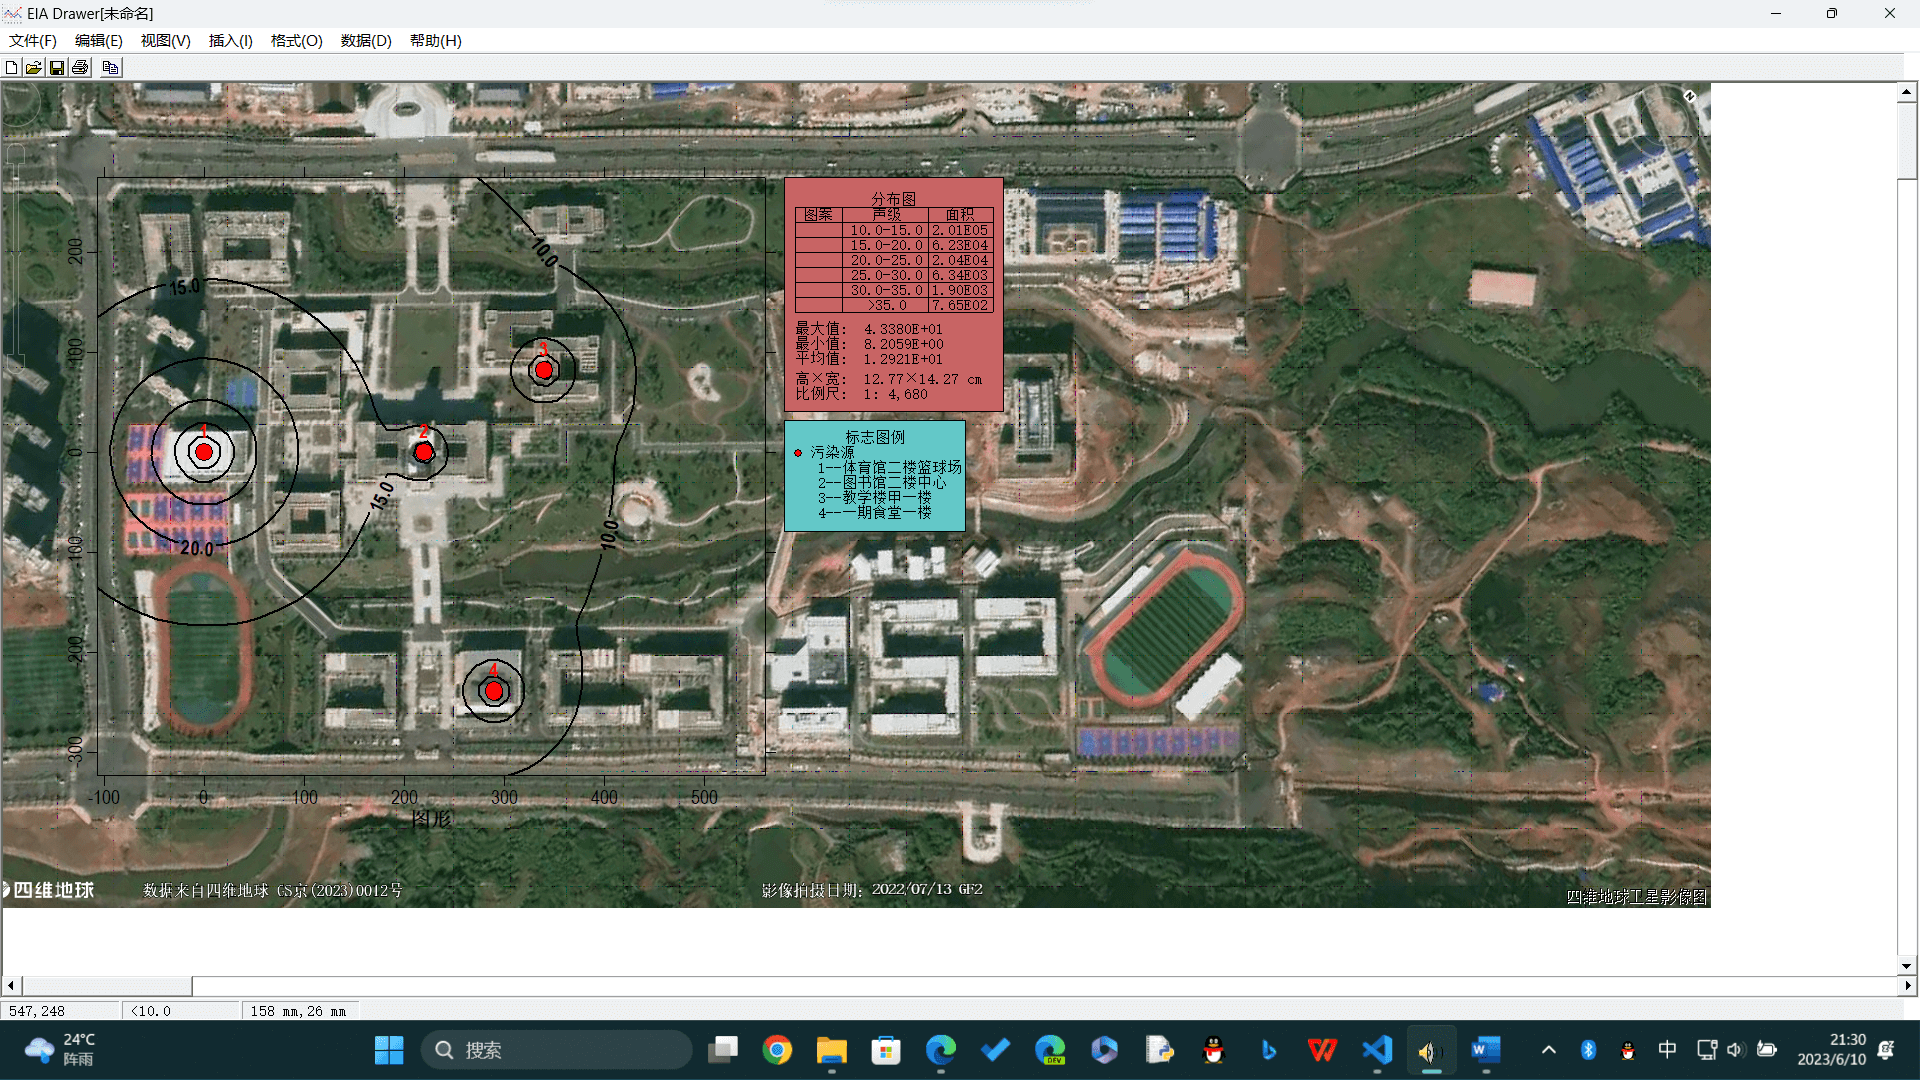
\includegraphics[width=0.8\textwidth]{figures/acoustic_step6-2.png}
            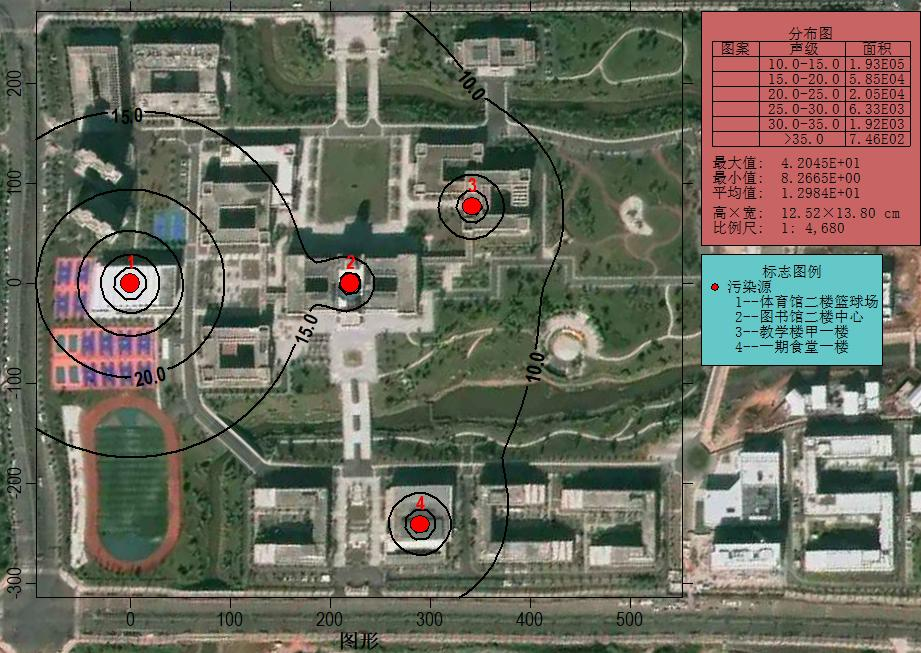
\includegraphics[width=0.8\textwidth]{figures/Campus noise attenuation plot-nighttime.jpg}
            \caption{夜}
        \end{subfigure}
        \caption{EIAN-校园噪声衰减图}
    \end{figure}
\end{enumerate}


\subsubsection{SCV 文件生成}
将生成的噪声衰减结果(如图 \ref{fig:Generate noise attenuation results})复制并保存到Excel中,然后将其转换为Sufer软件要求的导入格式(A列应包含X坐标,B列应包含Y坐标,C列应包含相应的噪声衰减值),就可以开始绘制噪声衰减图了。

\begin{figure}[H]
    \centering
    \begin{tikzpicture}
        \draw (1.2,0) rectangle node[midway] {$X$} (4,-1);
        \draw (0,-1.2) rectangle node[midway] {$Y$} (1,-4);
        \draw (1.2,-1.2) rectangle node[midway] {$Z$} (4,-4);
        \node[above] at (2,0.2) {原数据格式};
    \end{tikzpicture}
    \quad
    \tikz\draw[-stealth] (0,0) ++(0,2) -- ++(2,0) node[midway, above] {转换};
    \quad
    \begin{tikzpicture}
        \draw (0,0) rectangle node[midway] {$X$} (1,-4);
        \draw (1.2,0) rectangle node[midway] {$Y$} (2.2,-4);
        \draw (2.4,0) rectangle node[midway] {$Z$} (3.4,-4);
        \node[above] at (1.7,0.2) {目标CSV格式};
    \end{tikzpicture}
\end{figure}

由于在选择预测范围时选择了较大的区域:$(-94, -314)$ 到 $(552, 272)$,并且步长设置为每隔10米生成一次计算结果,所以最终得到的噪声衰减结果会非常庞大,数据总数为$X \times Y = 66 \times 60 = 3960$个。手动复制和粘贴来修改这么多数据的格式将会非常繁琐,因此我编写了一个小的Python程序来完成这个格式转化的任务。

\begin{lstlisting}[caption={将excel数据按要求转为csv.py}, label={lst:python_code}]
import pandas as pd
import csv

def extract_data(excel_file, sheet_index, csv_filename):
    # 提取数据和标题
    data = excel_file.parse(excel_file.sheet_names[sheet_index], header=0, index_col=0)
    x_title = data.columns.tolist()  # X坐标数组
    y_title = data.index.tolist()  # Y坐标数组
    data_values = data.values.tolist()  # 坐标值Z二维数组
    # 重新排列数据
    xyz = [[], [], []]
    for x in x_title:
        xyz[0].extend([x] * len(y_title))  # 录入X坐标
        xyz[1].extend(y_title)  # 录入Y坐标
        for each in range(len(data_values)):  # 录入相应坐标(X,Y)的Z值
            xyz[2].append(data_values[each][x_title.index(x)])
    # 创建CSV文件并写入数据
    with open(csv_filename, 'w', newline='') as csvfile:
        writer = csv.writer(csvfile)
        for row in zip(*xyz):
            writer.writerow(row)  # 列向写入数据
    print(csv_filename, "已生成CSV文件!")

# 读取Excel文件,并提取两个工作表(昼/夜)的数据
excel_file = pd.ExcelFile('校园噪声衰减数据.xlsx')  # Excel文件与.py路径同源
extract_data(excel_file, 0, 'daytime_xyz.csv')
extract_data(excel_file, 1, 'nighttime_xyz.csv')    
\end{lstlisting}

运行上述代码,我得到了 daytime_xyz.csv 和 nighttime_xyz.csv 文件,那么就可以开始下一步: Sufer 软件的使用。


\subsubsection{Sufer 操作步骤}
\begin{enumerate}
    \item Surfer 预处理生成 .grd 文件
    \begin{enumerate}[label=\arabic*)]
        \item 网格 $\rightarrow $ 数据 $\rightarrow $ 打开生成的 csv 文件;
        \begin{figure}[H]
            \centering
            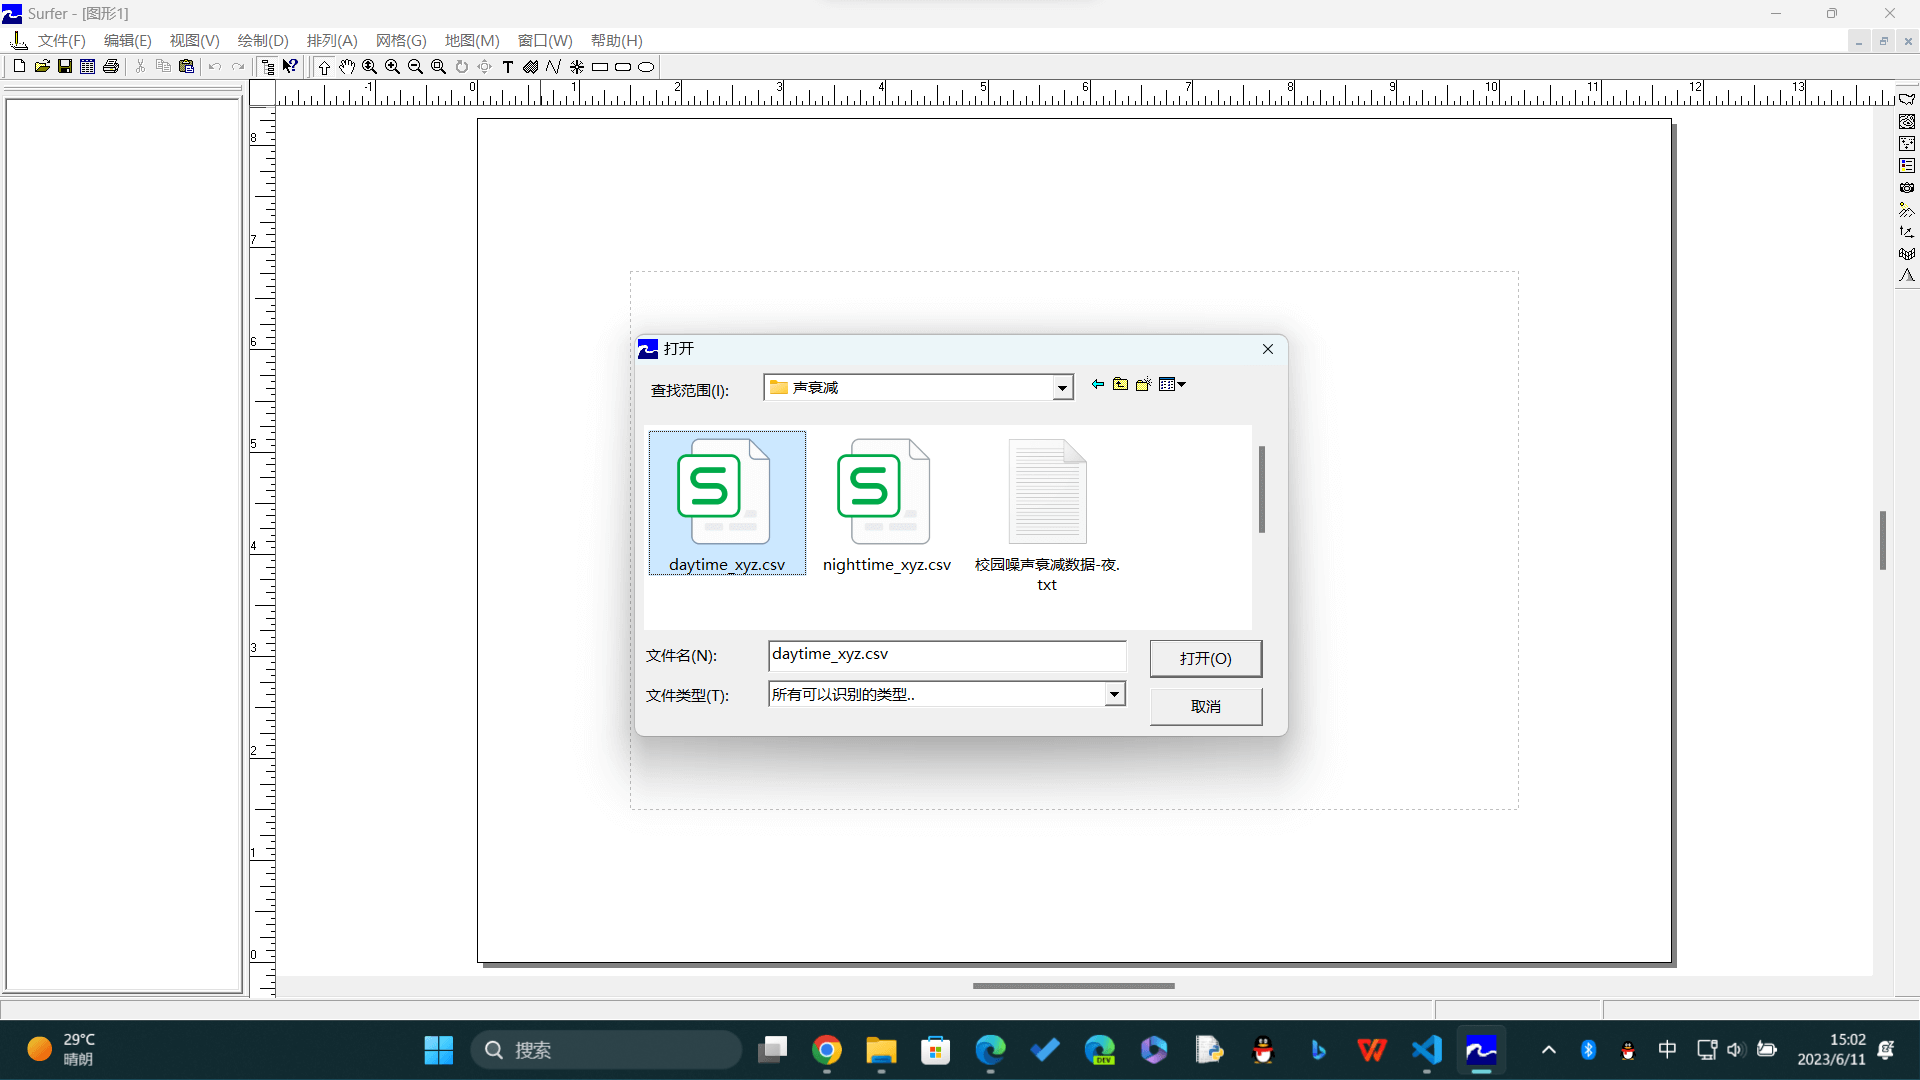
\includegraphics[width=0.8\textwidth]{figures/Sufer_step1-1.png}
            \caption{打开生成的 csv 文件}
        \end{figure}
        \item 网格化数据的导入(默认即可)。
        \begin{figure}[H]
            \centering
            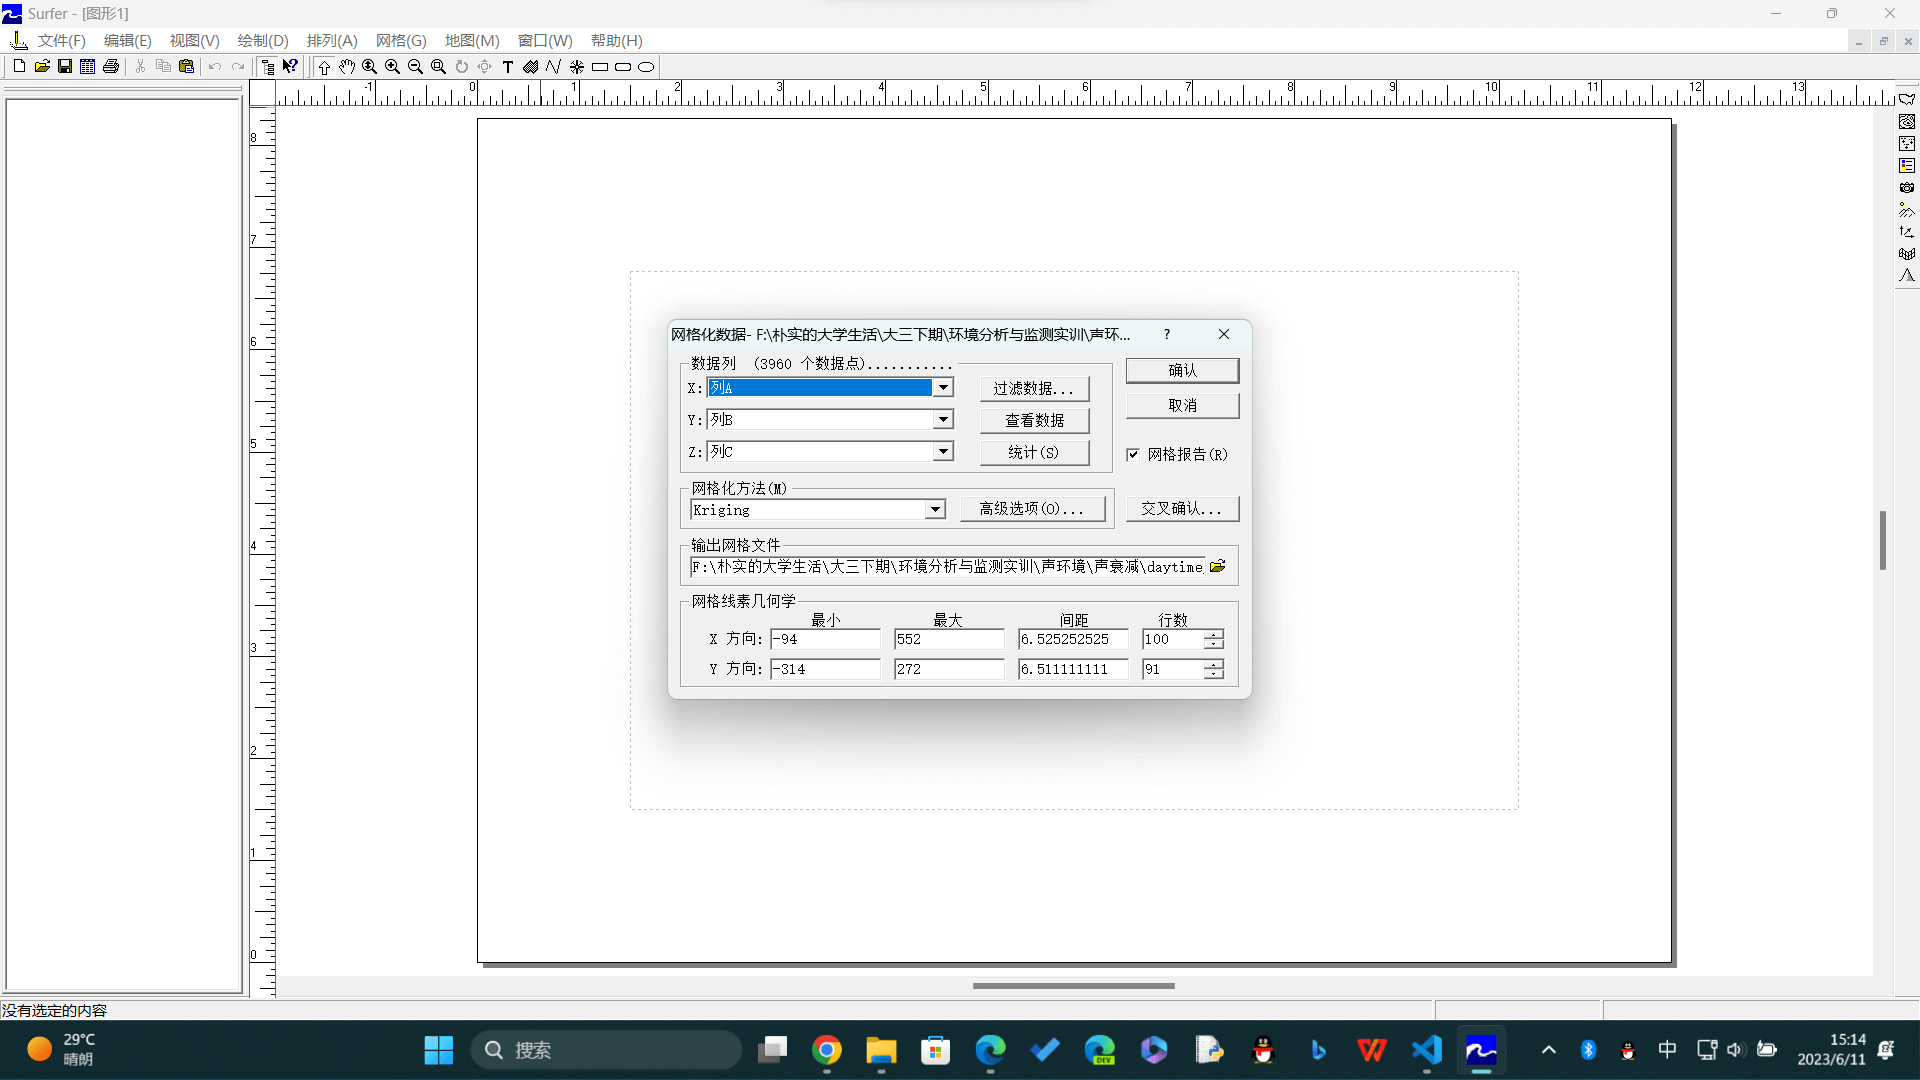
\includegraphics[width=0.8\textwidth]{figures/Sufer_step1-2.png}
            \caption{网格化数据导入设置}
        \end{figure}
    \end{enumerate}

    \item 画等值线图
    \begin{enumerate}[label=\arabic*)]
        \item 地图 $\rightarrow $ 等值线图 $\rightarrow $ 新建等值线图;
        \item 打开网格数据,选择刚才用 Excel 生成的 .grd 数据;
        \begin{figure}[H]
            \centering
            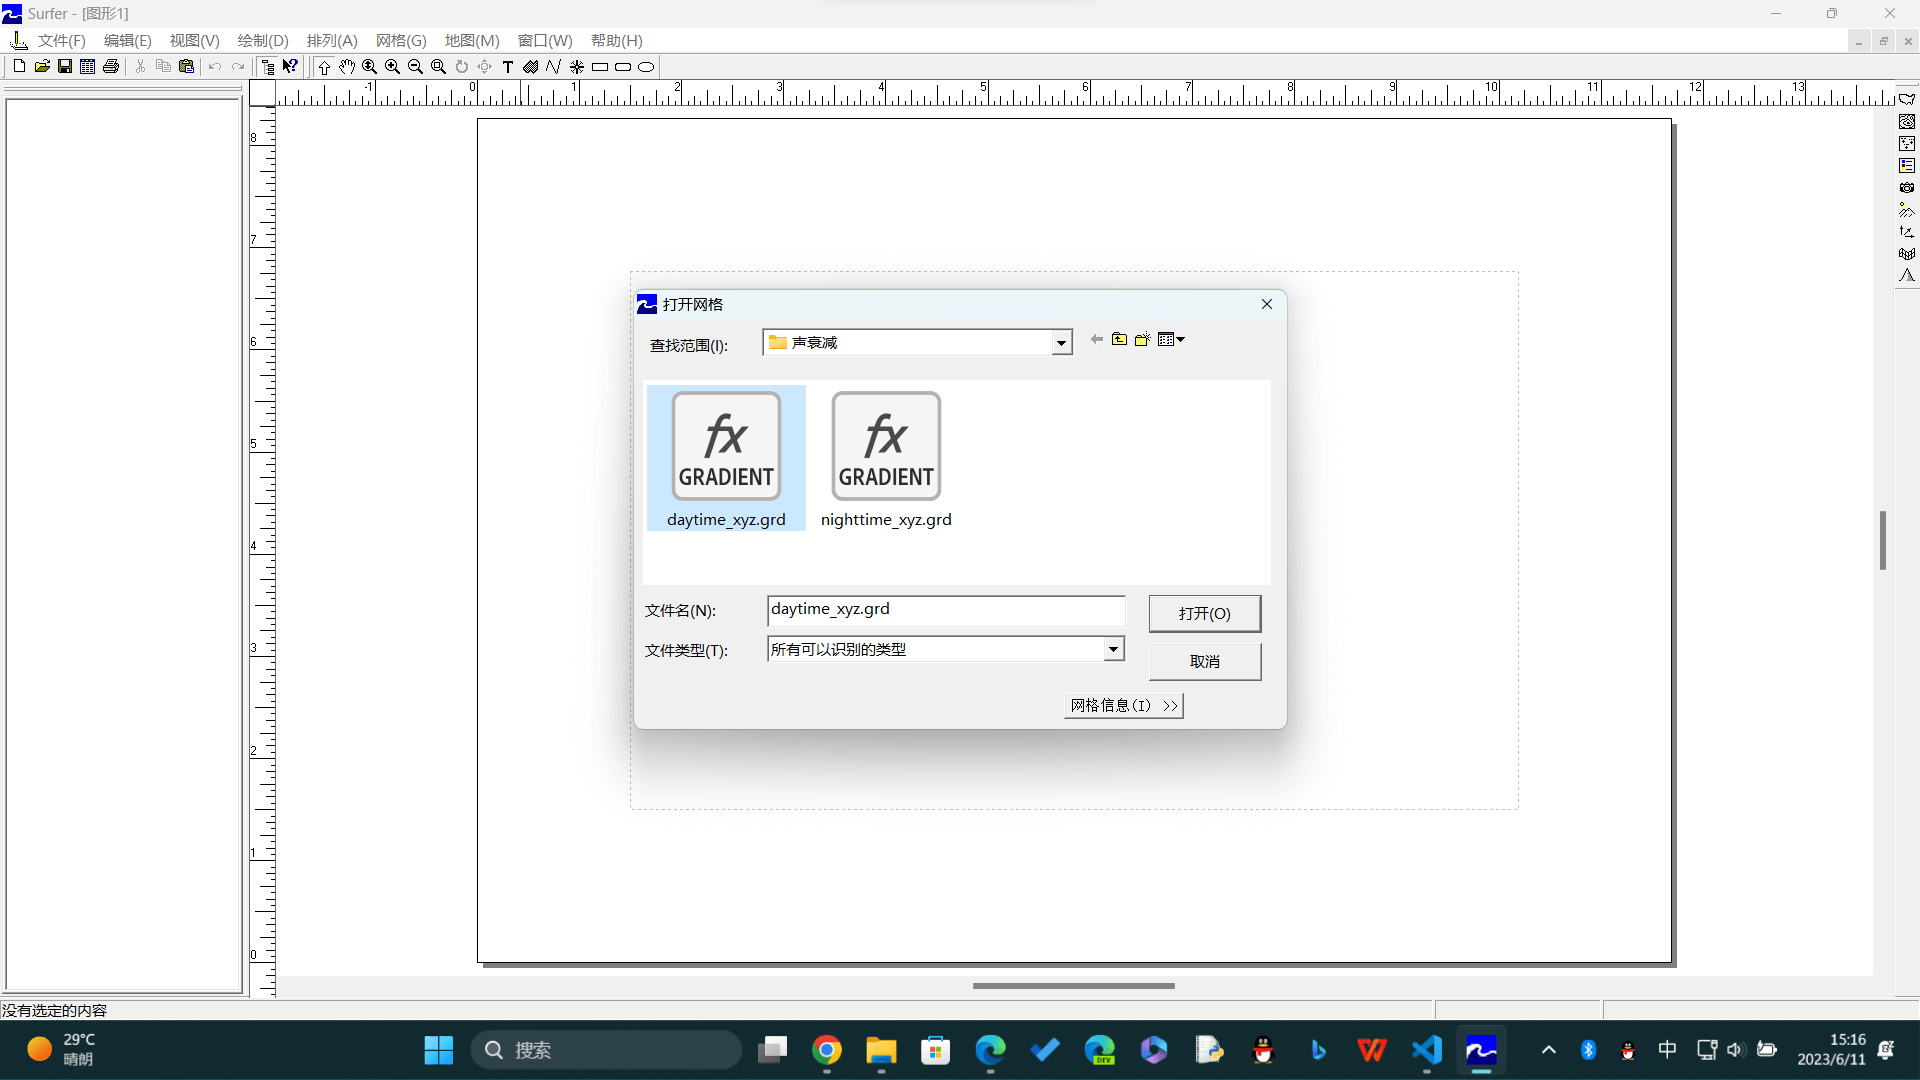
\includegraphics[width=0.8\textwidth]{figures/Sufer_step2-1.png}
            \caption{导入 .grd 数据}
        \end{figure}
        \item 一张朴实无华的等值线图就绘制完成。
        \begin{figure}[H]
            \centering
            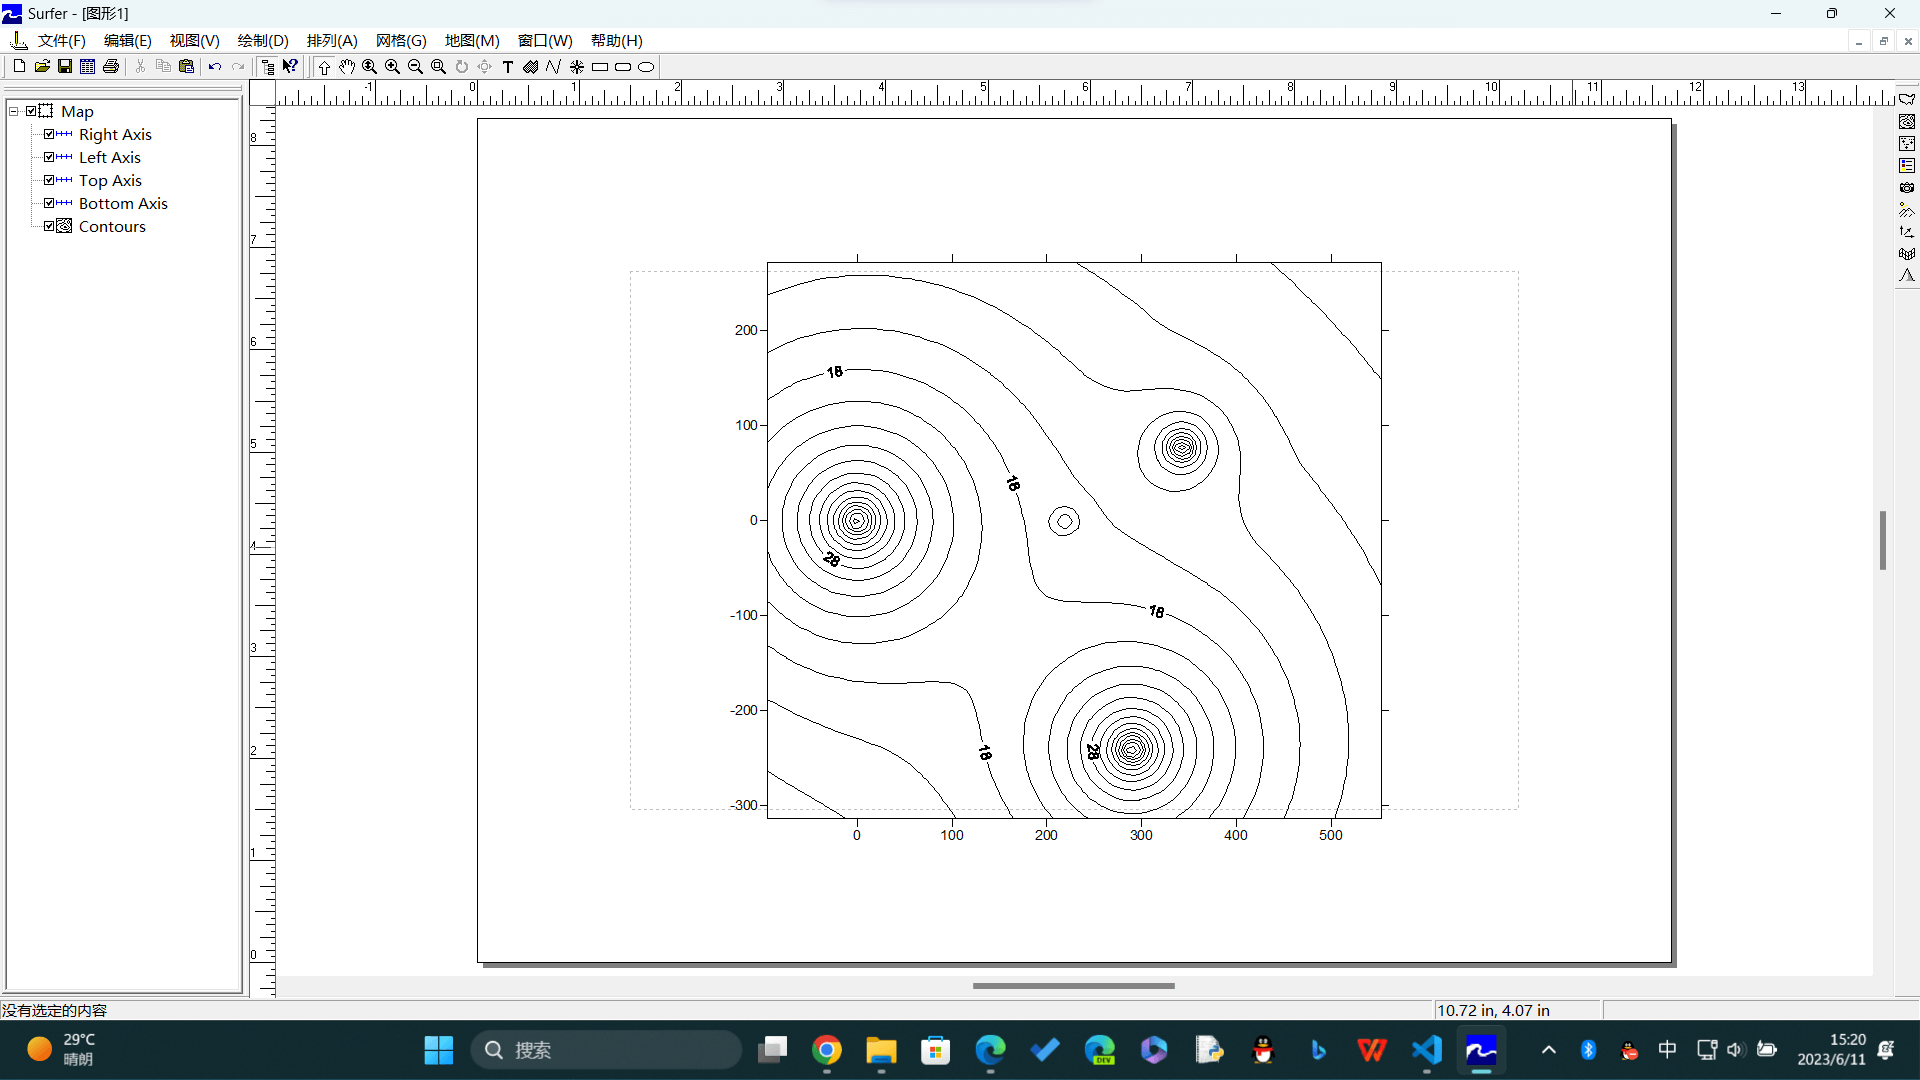
\includegraphics[width=0.8\textwidth]{figures/Sufer_step2-2.png}
            \caption{初始样式等声值线图}
        \end{figure}
    \end{enumerate}

    \item 等声值线图优化
    \begin{enumerate}[label=\arabic*)]
        \item 右键点击图片,打开“属性”;
        \item 依次将填充等值线和平滑中的选项勾选:
        \begin{itemize}
            \item 填充等值线(F)
            \item 平滑等值线(s)
            \item 颜色比例(C)
            \item 程度(M):高
        \end{itemize}
        \begin{figure}[H]
            \centering
            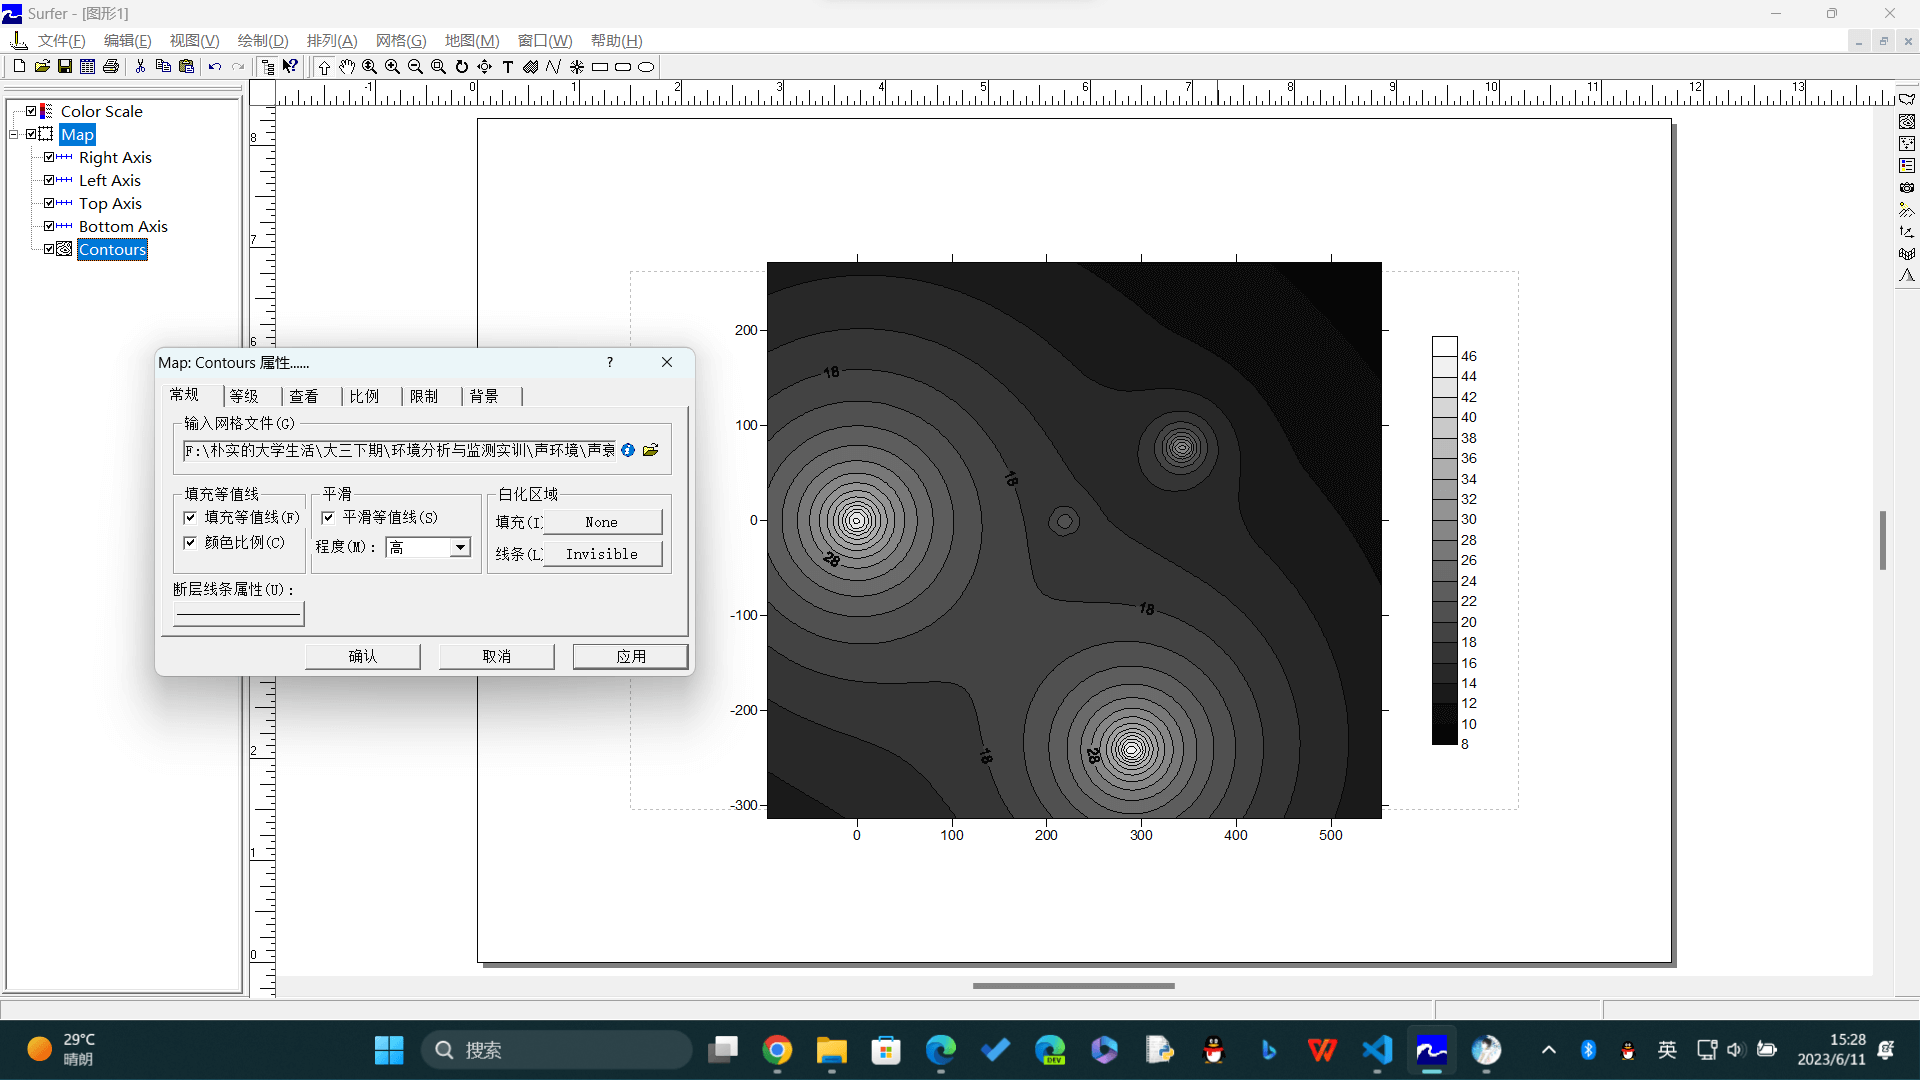
\includegraphics[width=0.8\textwidth]{figures/Sufer_step3-1.png}
            \caption{修改常规数值}
        \end{figure}

        \item 等级 $\rightarrow $ 填充
        \begin{itemize}
            \item 前景色: White \fcolorbox{black}{white}{\phantom{None}} Blue Violet \fcolorbox{black}{blueviolet}{\phantom{None}}
            \item 其余保持默认
        \end{itemize}
        \begin{figure}[H]
            \centering
            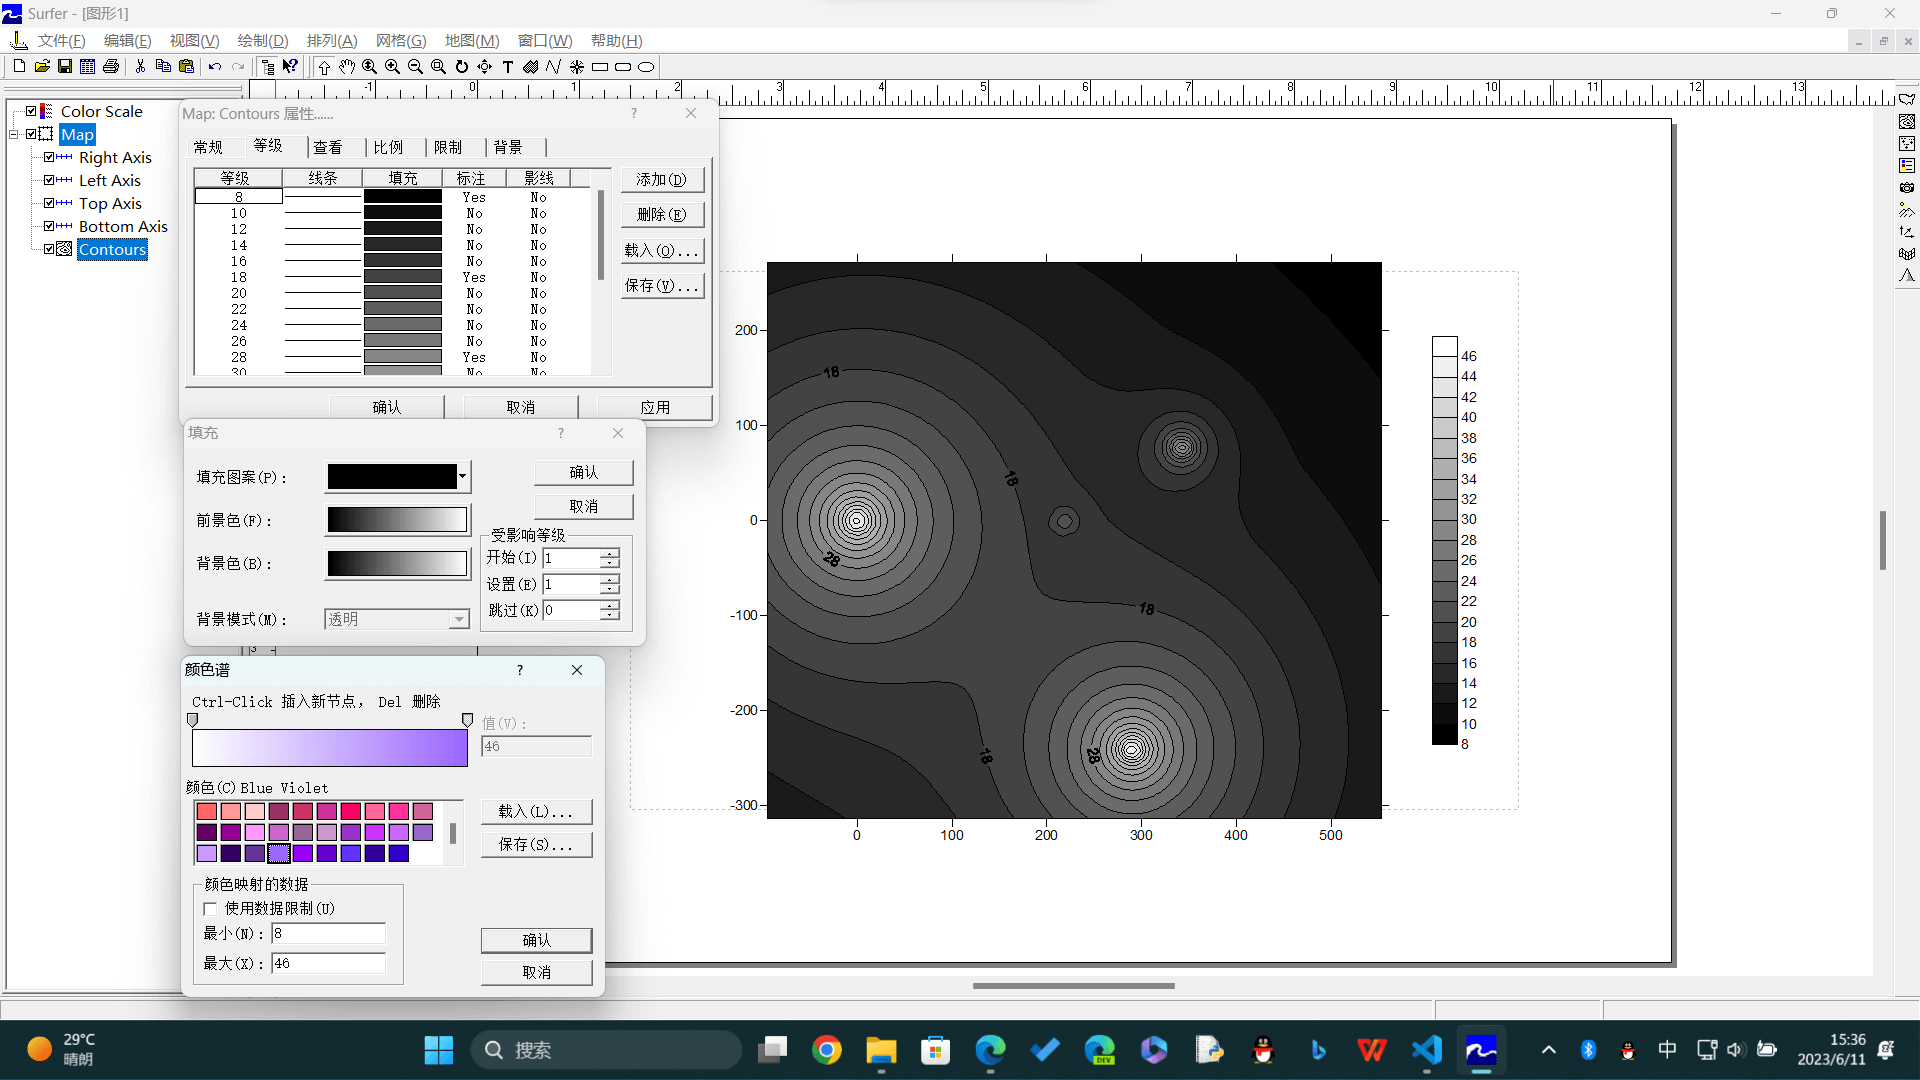
\includegraphics[width=0.8\textwidth]{figures/Sufer_step3-2.png}
            \caption{修改图形颜色}
        \end{figure}

        \item 等级 $\rightarrow $ 等级
        \begin{itemize}
            \item 间距:3
            \item 其余保持默认
        \end{itemize}
        \begin{figure}[H]
            \centering
            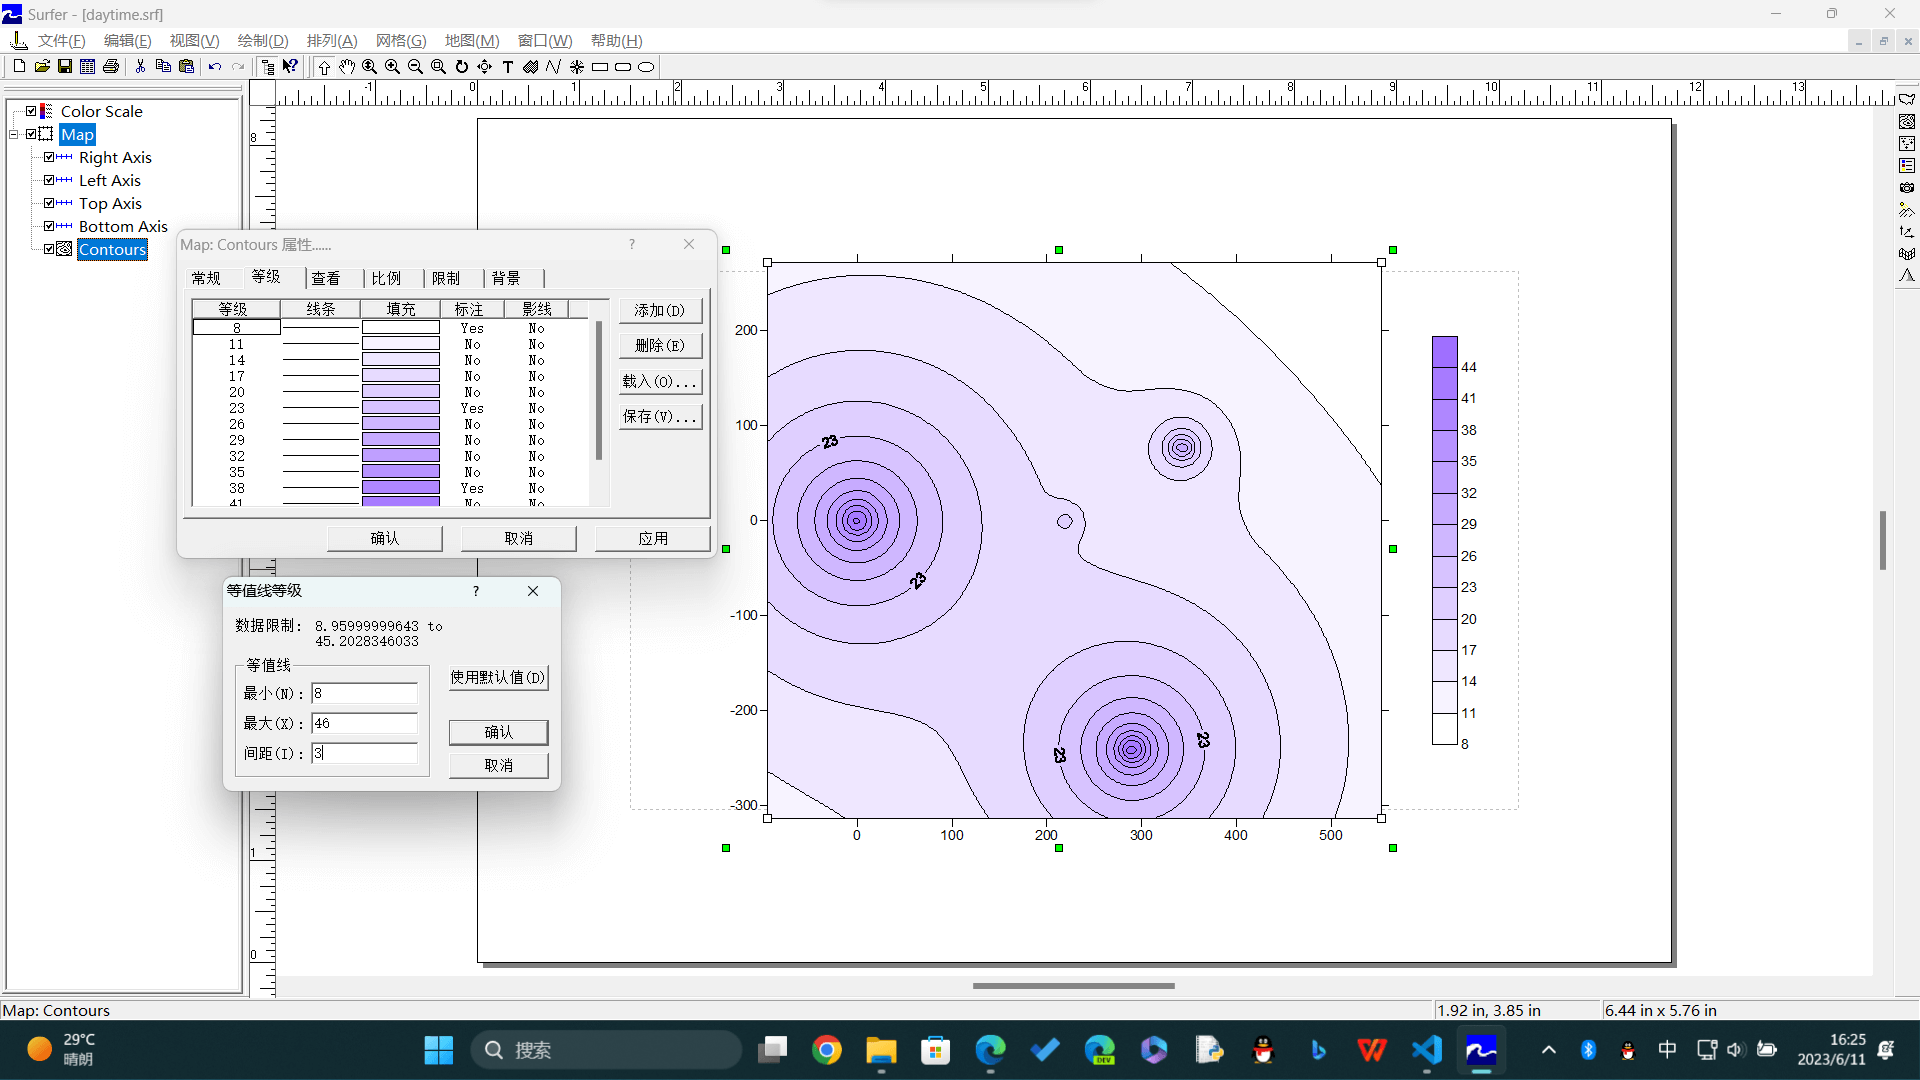
\includegraphics[width=0.8\textwidth]{figures/Sufer_step3-3.png}
            \caption{修改等级间距}
        \end{figure}

        \item 完成优化,获得一张全新而又优美且富有个人特色的等声值线图。
        \begin{figure}[H]
            \centering
            \begin{subfigure}[h]{\textwidth}
                \centering
                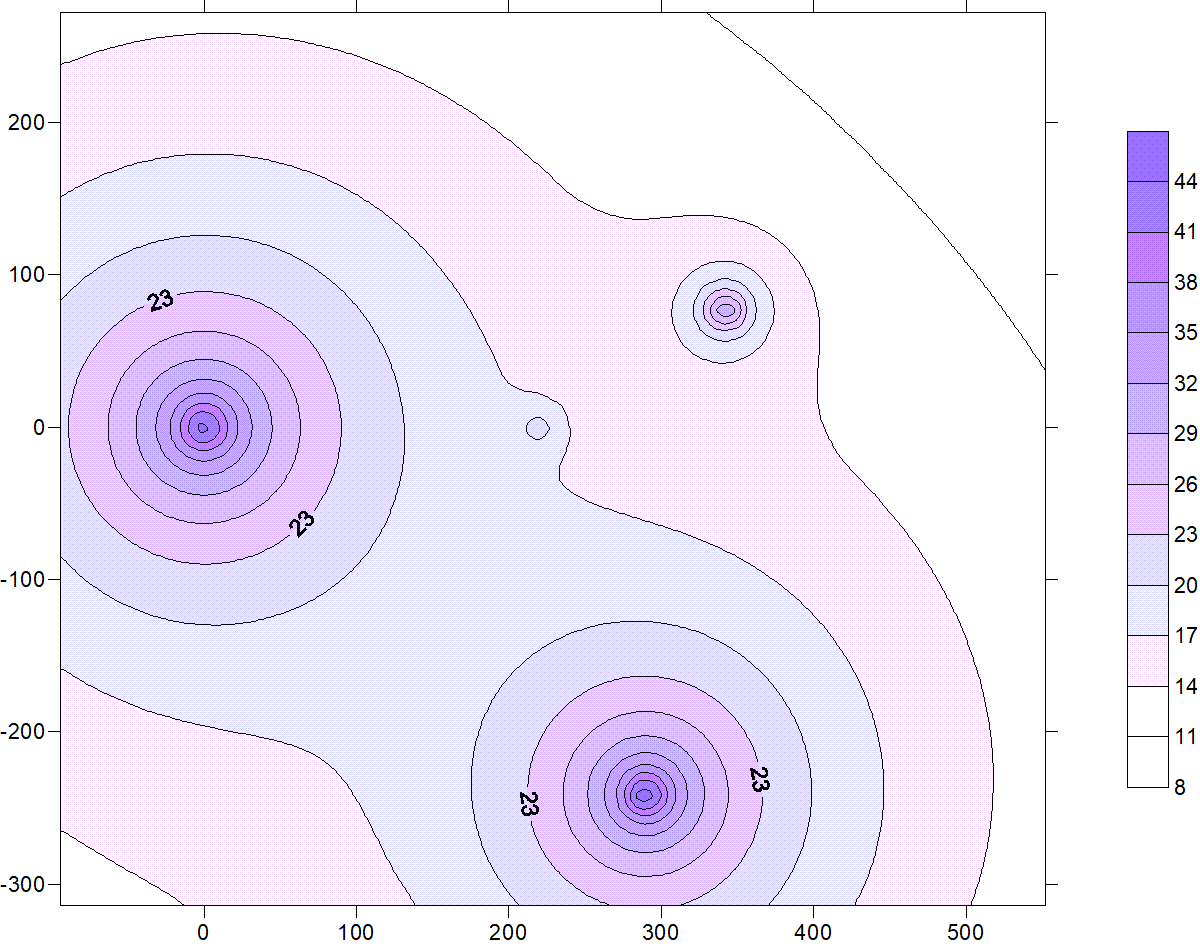
\includegraphics[width=0.8\textwidth]{figures/Campus noise attenuation plot-daytime.png}
                \caption{昼}
            \end{subfigure}
            \begin{subfigure}[h]{\textwidth}
                \centering
                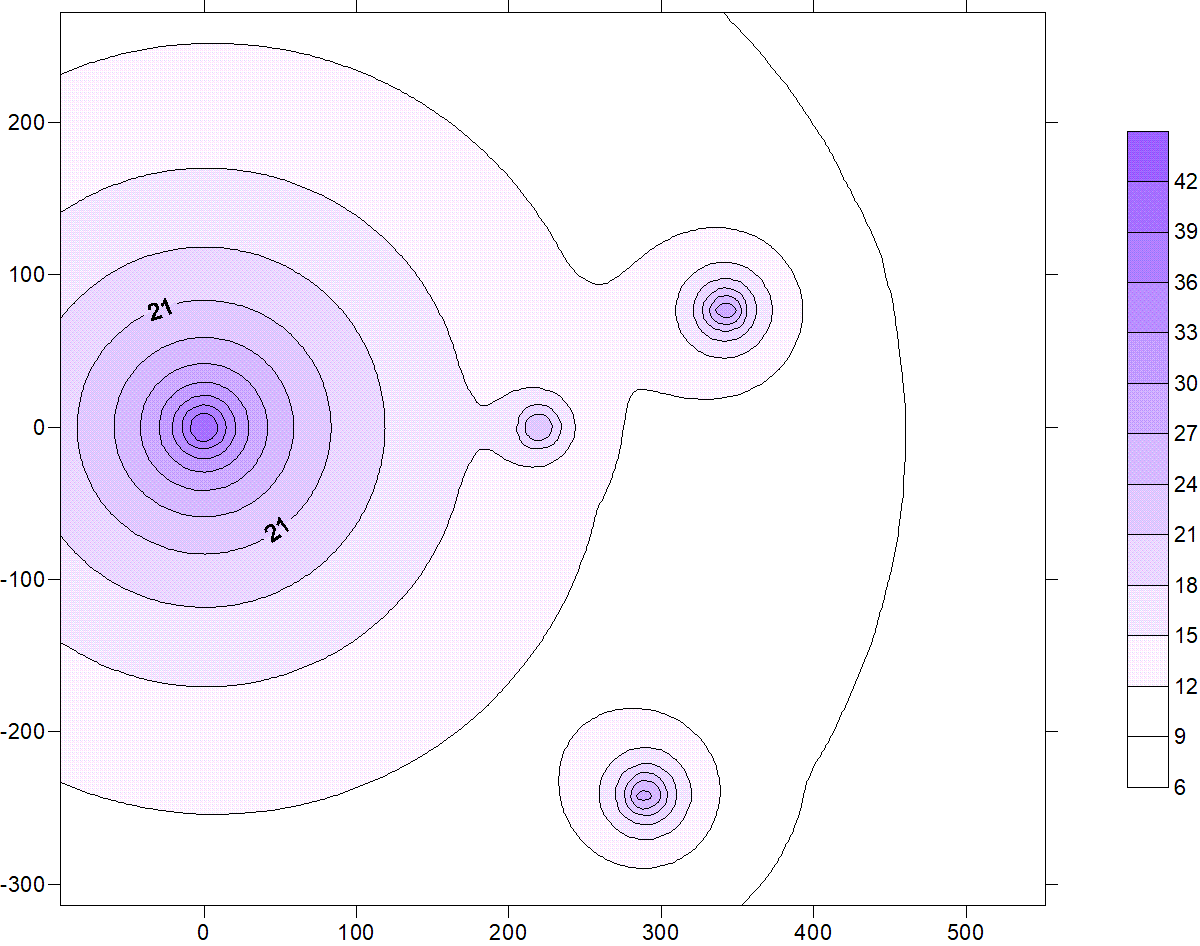
\includegraphics[width=0.8\textwidth]{figures/Campus noise attenuation plot-nighttime.png}
                \caption{夜}
            \end{subfigure}
            \caption{Sufer-校园昼夜噪声衰减等声值线图}
            \label{fig:Sufer-Isoacoustic line diagram of campus day and night noise attenuation}
        \end{figure}
    \end{enumerate}
\end{enumerate}


\subsubsection{评价分析}
由公式 \ref{eq:Geometric divergence attenuation calculation of point sound sources} 可得,当已知几何发散引起的衰减 $A_{div}$ dB(A),则可以反向求得衰减距离:
\begin{equation}
    r = r_0 \cdot 10^{0.05A}
\end{equation}
因为声环境监测记录的参考位置距声源的距离为 $r_0 = 1$ m,则
\begin{align*}
    r = 10^{0.05A}
\end{align*}
再根据表 \ref{tab:Summary of monitoring records} 中的数据和表 \ref{tab:Ambient noise limits} 中的环境噪声限值,可以计算出噪声达标距离,如下表 \ref{tab:Attenuation attainment distance} 所示:
\begin{table}[H]
    \centering
    \caption{衰减达标距离}
    \resizebox{\textwidth}{!}{
    \begin{tabular}{|c|c|c|c|c|c|c|}
    \multicolumn{7}{r}{单位:dB(A)} \\
    \hline
    \textbf{地点} & \textbf{时间} & \textbf{监测日期} & \textbf{昼夜} & \textbf{标准限值} & \textbf{Leq} & \textbf{衰减达标(m)} \\
    \hline
    \multirow{4}*{教学楼甲一楼} & \multirow{2}*{$9:00-10:00$} & 2023/6/7 & 昼     & 55.0  & 54.1  &  \\
    \cline{3-7}          &       & 2023/6/8 & 昼     & 55.0  & 51.9  &  \\
    \cline{2-7}          & \multirow{2}*{$19:30-20:30$} & 2023/6/6 & 夜     & 45.0  & 50.2  & 1.820  \\
    \cline{3-7}          &       & 2023/6/7 & 夜     & 45.0  & 52.6  & 2.399  \\
    \hline
    \multirow{4}*{体育馆二楼篮球场} & \multirow{2}*{$10:30-11:30$} & 2023/6/7 & 昼     & 55.0  & 70.4  & 5.888  \\
    \cline{3-7}          &       & 2023/6/8 & 昼     & 55.0  & 69.8  & 5.495  \\
    \cline{2-7}          & \multirow{2}*{$20:00-21:00$} & 2023/6/6 & 夜     & 45.0  & 68.8  & 15.488 \\
    \cline{3-7}          &       & 2023/6/7 & 夜     & 45.0  & 65.7  & 10.839 \\
    \hline
    \multirow{4}*{图书馆二楼中心} & \multirow{2}*{$9:30-10:30$} & 2023/6/7 & 昼     & 55.0  & 42.8  &  \\
    \cline{3-7}          &       & 2023/6/8 & 昼     & 55.0  & 43.8  &  \\
    \cline{2-7}          & \multirow{2}*{$21:00-22:00$} & 2023/6/6 & 夜     & 45.0  & 49.2  & 1.622\footnotemark  \\
    \cline{3-7}          &       & 2023/6/7 & 夜     & 45.0  & 43.6  &  \\
    \hline
    \multirow{4}*{一期食堂一楼} & \multirow{2}*{$11:30-12:30$} & 2023/6/7 & 昼     & 55.0  & 68.8  & 4.898  \\
    \cline{3-7}          &       & 2023/6/8 & 昼     & 55.0  & 68.6  & 4.786 \\
    \cline{2-7}          & \multirow{2}*{$22:00-23:00$} & 2023/6/6 & 夜     & 45.0  & 52.3  & 2.317  \\
    \cline{3-7}          &       & 2023/6/7 & 夜     & 45.0  & 50.2  & 1.820  \\
    \hline
    \end{tabular}}
    \label{tab:Attenuation attainment distance}
\end{table}
\footnotetext{由于2023年6月6日当天气温较高,图书馆在晚上开启了空调系统,这一举措旨在为人们提供舒适的环境。然而,由于空调系统的运行,从21:00至22:00期间记录的等效A声级Leq与随后在2023年6月7日晚上进行的监测结果相比较高。这差异也成为了超过标准限值范围的直接原因。}


根据图 \ref{fig:Sufer-Isoacoustic line diagram of campus day and night noise attenuation} 所示,
昼间时,体育馆二楼篮球场和一期食堂一楼对周围环境的影响最为显著,其辐射范围最广。体育馆二楼篮球场主要在上午的第3至4节课($10:25-11:50$)产生噪声,这是由室内体育篮球课引起的。而一期食堂一楼则主要受同学们就餐和相互交谈所产生的无序声音影响。
夜间时,只有体育馆二楼篮球场仍会产生噪声,主要是因为同学们在夜间进行体育锻炼,例如打篮球或打羽毛球等活动。

虽然体育馆二楼篮球场和一期食堂一楼是两个主要的噪声来源,其周围分别有教师公寓和学生宿舍等敏感区域,但这些主要噪声源的发声时段并不会干扰周围敏感区域的正常作息。此外,体育馆二楼篮球场内部设有减噪设备,因此这些噪声源并不构成问题。
此外,根据表 \ref{tab:Attenuation attainment distance} 所示,即使噪声传播到敏感区域,其声音衰减已经达到了规定的标准范围,因此对周围环境的影响不大。


\subsection{小结及建议}
但学校是一个比较需要安静的地方,还是可以通过噪声源管理、减噪设备改进、敏感点保护、定期噪声评估以及意识提高等措施,来进一步改善噪声评价并提供更好的噪声环境。
\begin{enumerate}
    \item 噪声源管理:对于体育馆二楼篮球场和一期食堂一楼这两个主要噪声源,可以采取一些管理措施,以降低其对周围环境的影响。例如,在体育馆二楼篮球场上课期间,可以考虑使用更加静音的篮球设备,或者在场地周围设置隔音措施,减少噪声传播。对于一期食堂一楼,可以考虑优化空间设计,采用吸音材料或隔音屏障,减少就餐和交谈声音的扩散。
    \item 减噪设备改进:尽管体育馆二楼篮球场已经安装了减噪设备,但可以进一步评估其性能并考虑改进。定期维护和检查减噪设备的运行状况,确保其有效工作。如果发现存在问题或技术更新,可以考虑升级设备,以提供更好的噪声控制效果。
    \item 增加敏感点保护:尽管噪声源的发声时段不会干扰周围的敏感点,但可以进一步加强对敏感点的保护措施。例如,在教师公寓和学生宿舍等敏感区域内安装隔音设施,以减少噪声的传播和干扰。此外,定期监测敏感区域的噪声水平,确保其在规定的标准范围内。
    \item 定期噪声评估:定期进行噪声评估是必要的,以监测噪声水平的变化和影响范围。根据评估结果,可以及时调整管理措施或采取进一步的噪声控制措施。噪声评估可以包括现场测量和主观问卷调查等方法,以全面了解噪声问题并制定相应的对策。
    \item 提高意识和宣传:加强对噪声问题的宣传和意识提高,促使全校师生共同关注噪声环境,提醒人们在使用体育馆和食堂等场所时注意噪声控制,培养良好的噪声行为习惯。
\end{enumerate}

这些建议和措施有助于减少噪声对周围环境和敏感点的影响,提升整体的居住和学习体验、创造出更宜人的噪声环境,为师生提供更好的学习和生活条件。
